%*******10********20********30********40********50********60********70********80

% For all chapters, use the newdefined chap{} instead of chapter{}
% This will make the text at the top-left of the page be the same as the chapter

\chap{Σχεδιασμός \& Υλοποίηση Εφαρμογής} \label{c:design}



Στο κεφάλαιο \ref{c:2}, διερευνήσαμε το πεδίο της επαυξημένης πραγματικότητας και τις μαθηματικές αρχές από τις οποίες διέπεται. Παρουσιάσαμε επίσης τη χρησιμότητα της ενσωμάτωσης δυνατοτήτων αναγνώρισης χειρονομιών σε εφαρμογές, καθώς και ερευνητικές εργασίες σχετικές με τη παρούσα διπλωματική εργασία.


Όπως αναφέρθηκε, πολλές εφαρμογές επαυξημένης πραγματικότητας έχουν αναπτυχθεί στον τομέα των βιντεοπαιχνιδιών. Στις παρακάτω ενότητες θα πραγματοποιηθεί ανάλυση των μεθόδων που αναπτύχθηκαν για την δημιουργία ενός σκακιού επαυξημένης πραγματικότητας, όπου ο χρήστης μπορεί να χειριστεί εικονικά πιόνια μόνο με τα χέρια του με χειρονομίες "τσιμπήματος". Αρχικά θα παρουσιαστούν τα εργαλεία και ο αισθητήρας που χρησιμοποιήθηκαν, καθώς και η πειραματική εγκατάσταση για τις δοκιμές της εφαρμογής. Τα επόμενα στάδια περιλαμβάνουν την ανάλυση της διαδικασίας βαθμονόμησης και την παρουσίαση των μεθόδων ανίχνευσης της θέσης του τσιμπήματος και χειρισμού των εικονικών αντικειμένων. Γίνεται λόγος για τη διαδικασία ενσωμάτωσης μιας μηχανής σκακιού στην εφαρμογή, ενώ τέλος, παρουσιάζεται η αξιοποίηση μιας μεθόδου που βοηθά στην αντιμετώπιση του προβλήματος της απόκρυψης εικονικών και πραγματικών αντικειμένων.





Η ανάπτυξη και η υλοποίηση ενός συστήματος επαυξημένης πραγματικότητας προϋποθέτει κατά το σχεδιασμό, τη λήψη αποφάσεων σχετικά με τις επιλογές για την υλοποίηση. Οι επιλογές τόσο σε software όσο και σε hardware πρέπει να εξεταστούν πριν ξεκινήσει η διαδικασία της ανάπτυξης. Ορισμένες επιλογές που παίζουν σημαντικό ρόλο στο σχεδιασμό έχουν να κάνουν με τη μέθοδο ανίχνευσης, το είδος των marker που θα χρησιμοποιηθούν, τον τρόπο επαύξησης, και το λογισμικό που θα υλοποιηθεί. Άλλοι περιορισμοί που πρέπει να ληφθούν υπόψη αφορούν το κόστος και τη δυσκολία ενσωμάτωσης.


Επιλέχθηκε η παρουσίαση των αλγορίθμων που αναπτύχθηκαν και θα παρουσιαστούν στη συνέχεια να μη γίνει με τη μορφή κειμένου, αλλά να παρουσιάστει με τη μορφή διαγραμμάτων ροής.




\section{Η Συσκευή Intel\textsuperscript{\textregistered} RealSense\texttrademark{} 3D F200 }



Η πλατφόρμα Intel\textsuperscript{\textregistered} RealSense\texttrademark{}, παλαιότερα γνωστή ως Intel\textsuperscript{\textregistered} Perceptual Computing, είναι μία πλατφόρμα που επιτρέπει την υλοποίηση τεχνικών αλληλεπίδρασης ανθρώπου-υπολογιστή με βάση τις χειρονομίες. Αποτελείται από μία σειρά 3D αισθητήρων και μία βιβλιοθήκη που απλοποιεί τη χρήση των αισθητήρων από προγραμματιστές λογισμικού. \cite{RealsenseCamera}


Η συγκεκριμένη τεχνολογία θεωρείται διάδοχος της τεχνολογίας του αισθητήρα Microsoft Kinect, με κύριο στόχο τη δημιουργία εφαρμογών για τεχνολογίες της αγοράς πέρα από τα βιντεοπαιχνίδια. Από το Μάρτιο του 2015, πολλοί κατασκευαστές φορητών υπολογιστών και tablets\cite{Realsenselaptops}, όπως οι Asus, HP, Dell, Lenovo, and Acer διαθέτουν συσκευές με ενσωματωμένο τον αισθητήρα Intel\textsuperscript{\textregistered} RealSense\texttrademark{}. 


Ένας τέτοιος αισθητήρας περιλαμβάνει τα παρακάτω 4 εξαρτήματα: 


\begin{itemize}
  \item 1 συμβατική κάμερα
  \item 1 προβολέα υπερύθρων ακτίνων laser (infrared laser projector)
  \item 1 κάμερα υπερύθρων
  \item 2 μικρόφωνα
\end{itemize}



Ο προβολέας υπερύθρων ακτίνων laser προβάλλει ένα πλέγμα στη σκηνή (σε υπέρυθρο φως που είναι αόρατο στο ανθρώπινο μάτι) και η κάμερα υπερύθρων το καταγράφει με στόχο να υπολογίσει πληροφορίες για το βάθος της σκηνής.
Τα μικρόφωνα επιτρέπουν τον εντοπισμό πηγών ήχου στο χώρο και την ακύρωση θορύβου παρασκηνίου.


Ανακοινώθηκαν 3 διαφορετικά μοντέλα αισθητήρων, με συγκεκριμένες ιδιότητες και προβλεπόμενη χρήση. 

\begin{description}
  \item[Intel\textsuperscript{\textregistered} RealSense\texttrademark{} 3D Camera (Front F200)] \hfill \\
  Πρόκειται για έναν αισθητήρα που μπορεί να συνδεθεί με φορητούς ή σταθερούς υπολογιστές και προορίζεται για χρήσεις όπως η αλληλεπίδραση με φυσικές χειρονομίες, η αναγνώριση προσώπου, οι τηλεδιασκέψεις, η 3D σάρωση και το gaming.
  
  \item[Intel\textsuperscript{\textregistered} RealSense\texttrademark{} Snapshot] \hfill \\
 Ο αισθηρήρας Snapshot προορίζεται για χρήση μέσω tablets και πιθανότατα smartphones. Η χρήση του περιλαμβάνει λήψη φωτογραφιών και ιδιότητες όπως επανεστίαση, υπολογισμοί αποστάσεων και φίλτρα κίνησης. 


  \item[Intel\textsuperscript{\textregistered}RealSense\texttrademark{} 3D Camera (Rear R200)] \hfill \\
  Το τρίτο είδος αισθητήρα της Intel προορίζεται για προσαρμογή στο πίσω μέρος συσκευών όπως το Microsoft Surface ή παρόμοιων tablets. Δεν είναι ακόμα διαθέσιμο στην αγορά, ωστόσο προορίζεται για εφαρμογές επαυξημένης πραγματικότητας, δημιουργία περιεχομένου και σάρωση αντικειμένων.
\end{description}




Στη συγκεκριμένη εργασία χρησιμοποιήσαμε το πρώτο είδος αισθητήρα, τη συσκευή Intel\textsuperscript{\textregistered} RealSense\texttrademark{} 3D F200, η οποία διατίθεται από την Intel\textsuperscript{\textregistered} μέσω ενός Development Kit στην τιμή των 99 δολλαρίων. Διαθέτει ανάλυση βάθους Full VGA, κάμερα RGB 1080p, εμβέλεια ανίχνευσης περίπου 0.2–1.2 μέτρα και συνδέεται μέσω USB 3.0 σε έναν υπολογιστή.


Ο αισθητήρας βάθους μέσω υπερύθρων προσφέρει καλύτερη αναγνώριση χειρονομιών από μία παραδοσιακή κάμερα. Μέσω του αισθητήρα της Intel, μπορούμε να προσθέσουμε δυνατότητες αναγνώρισης χειρονομιών σε ήδη υπάρχοντα συστήματα βιντεοπαιχνιδιών.
ενώ μας δίνεται η δυνατότητας να αξιοποιήσουμε τα χέρια μας ως χειριστήρια.

Η συσκευή RealSense\texttrademark{} 3D επιλέχθηκε για τις δυνατότητές της σε σχέση με άλλους αισθητήρες όπως το Microsoft Kinect, λόγω του μικρού μεγέθους και της δυνατότητας ανίχνευσης βάθους σε κοντινότερες αποστάσεις. Επίσης προσφέρει εύκολο χειρισμό των ακατέργαστων δεδομένων (raw data), καθώς επίσης μέσω του SDK προσφέρονται αλγόριθμοι για την εξαγωγή blobs, το φιλτράρισμα και τον καθορισμό παραμέτρων. 



\begin{figure}[H]
    \centering
    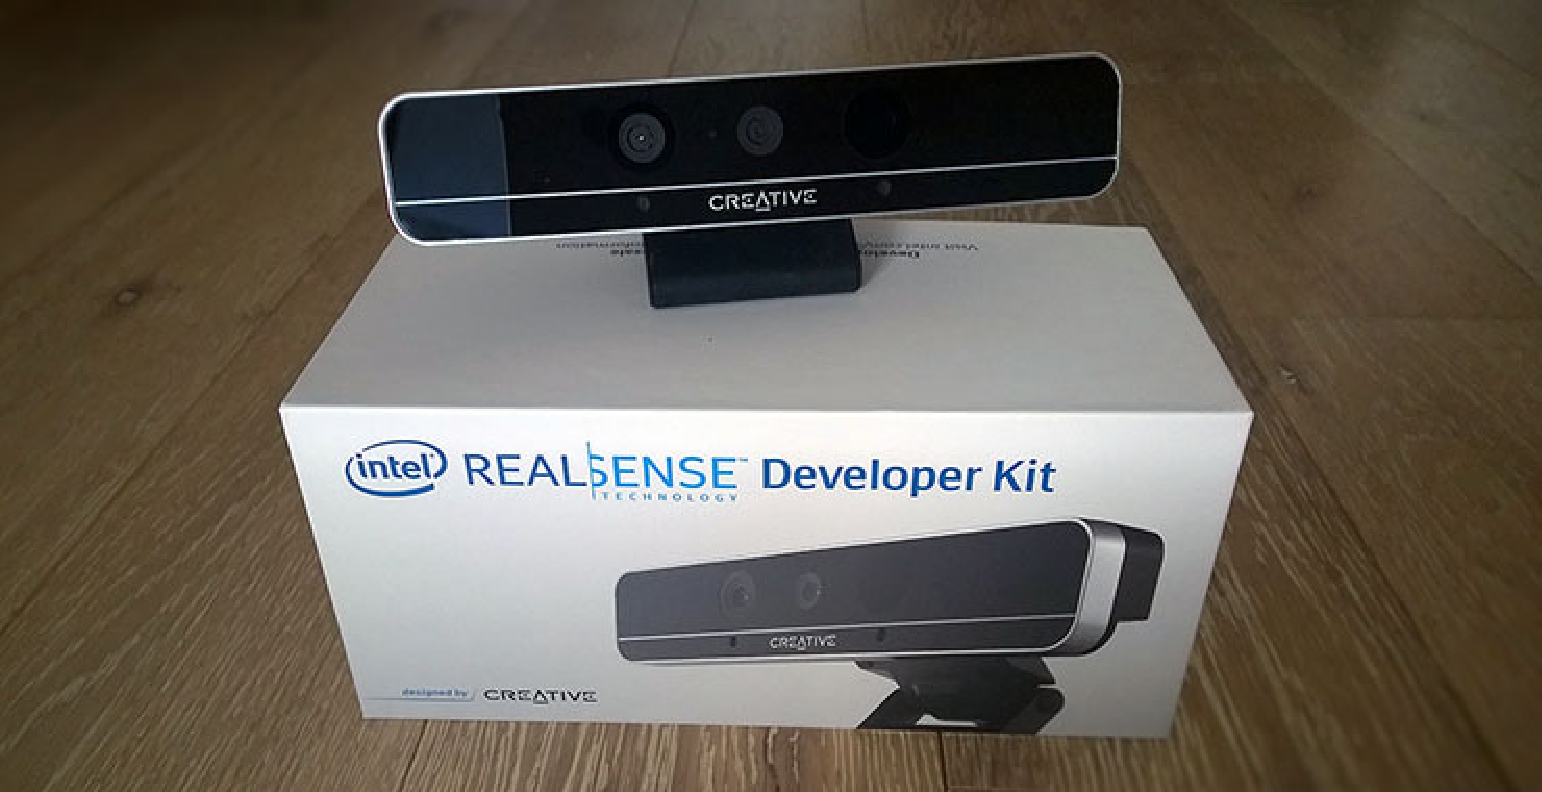
\includegraphics[scale=0.35, angle=0]{Files/Figures/RealSenseCamera.pdf}
    \caption[Η Συσκευή Intel\textsuperscript{\textregistered} RealSense\texttrademark{} 3D F200]{Η Συσκευή Intel\textregistered\ RealSense\texttrademark{} 3D F200}
    \label{fig:realsense}
\end{figure}



\section{Επιλογή Εργαλείων Ανάπτυξης}
%ARUCO,OPENCV,KLP


Πριν το σχεδιασμό μιας εφαρμογής επαυξημένης πραγματικότητας, η διαδικασία επιλογής των κατάλληλων βιβλιοθηκών και εργαλείων λογισμικού που θα χρησιμοποιηθούν, αποτελεί μία σημαντική πτυχή για την πετυχημένη υλοποίηση της εφαρμογής. 


Πέρα από την κατάλληλη επιλογή αισθητήρα χρώματος - βάθους,
πρέπει να επιλεγούν εργαλεία τα οποία θα είναι συμβατά με τον αισθητήρα και τις απαιτήσεις του. Πιο συγκεκριμένα, για τη σωστή λειτουργία του αισθητήρα απαιτείται υπολογιστική μονάδα με επεξεργαστή Intel\textsuperscript{\textregistered} Core\texttrademark{} τουλάχιστον 4ης γενιάς και λειτουργικό Windows 8.1 (64bit). Επιπλέον η υπολογιστική μονάδα πρέπει να διαθέτει θύρες USB 3.0 για τη σύνδεση με τον αισθητήρα, ενώ σαν γλώσσες προγραμματισμού υποστηρίζονται οι C++, JavaScript, C\#, Java και Processing.


Για τους παραπάνω λόγους, η υλοποίηση της εφαρμογής έλαβε μέρος σε ένα φορητό υπολογιστή  MacBook Pro με επεξεργαστή Intel\textsuperscript{\textregistered} Core\texttrademark{} i5 4278U (2.6GHz) με μνήμη RAM στα 16GB και λειτουργικό σύστημα Windows 8.1 Professional (64bit). Επίσης λόγω της πολυπλοκότητας υλοποίησης απαιτείται η χρήση πολλών διαφορετικών βιβλιοθηκών και η αξιοποίηση των χαρακτηριστικών τους. Για τον ευκολοτερο συνδυασμό των βιβλιοθηκών, χρησιμοποίηθηκε ως IDE το Visual Studio 2010.


Μεταξύ μιας ποικιλίας βιβλιοθηκών επαυξημένης πραγματικότητας, επιλέχθηκε η βιβλιοθήκη ArUco λόγω της απλότητάς της (ανίχνευση markers με μία μόνο γραμμή κώδικα C++) και της δυνατότητας δημιουργίας markerboards που επιτρέπουν την απρόσκοπτη ανίχνευσή τους. Η έκδοση που χρησιμοποιήθηκε (1.2.5) διαθέτει υποστήριξη για διαφορετικές πλατφόρμες (Java, C++, Python) και είναι καλά τεκμηριωμένη (documentation). Επιπλέον διαθέτει ελεύθερη άδεια προς χρήση σε σύγκριση με εργαλεία όπως αυτά που προσφέρουν άλλες εταιρίες όπως η Metaio. Το γεγονός ότι μπορεί εύκολα να συνδυαστεί με την OpenCV και την OpenGL είναι αυτό που συνετέλεσε κυρίως στην επιλογή της.


Οι βιβλιοθήκες λογισμικού που αξιοποιήθηκαν εμφανίζονται παρακάτω:

\begin{description}


\item[OpenGL \& GLUT:] Πρόκειται για μία διαγλωσσική διεπαφή προγραμματισμού εφαρμογών που υποστηρίζει πολλές πλατφόρμες για την απεικόνιση 2D και 3D γραφικών. Χρησιμοποείται στην εφαρμογή μας για την απεικόνιση των εικονικών αντικειμένων πάνω στο βίντεο, το οποίο καταγράφει την πραγματική σκηνή. Παρά το γεγονός ότι θα μπορούσε να χρησιμοποιηθεί μία μηχανή βιντεοπαιχνιδιών όπως η Unity3D για την ευκολότερη διαχείριση των ιδιοτήτων των εικονικών αντικειμένων, επιλέξαμε τη χρήση της OpenGL, προκειμένου να κατανοηθούν οι βασικές τεχνικές που χρησιμοποιούνται στην ανάπτυξη εφαρμογών επαυξημένης πραγματικότητας.



\item[OpenCV (2.4.10):] Γνωστή βιβλιοθήκη προγραμματιστικών συναρτήσεων που έχουν ως στόχο την ανάπτυξη εφαρμογών υπολογιστικής όρασης και την επεξεργασία εικόνας και βίντεο. Η συγκεκριμένη βιβλιοθήκη ανοιχτού κώδικα σχεδιάστηκε για να είναι αποδοτική ώστε να υποστηρίζει εφαρμογές πραγματικού χρόνου, ενώ υποστηρίζει διάφορες πλατφόρμες όπως Windows, Linux, Mac OS X, iOS και Android και διαθέτει διεπαφές για τις γλώσσες C,C++ και Java. 


\item[Qt (5.4)]: Πρόκειται για ένα framework ανάπτυξης που υποστηρίζει πολλές πλατφόρμες για την δημιουργία εφαρμογών, διεπαφών χρηστών (UI) και συσκευών. Για την ανάπτυξη της εφαρμογής σκακιού επαυξημένης πραγματικότητας, χρησιμοποιήθηκαν μόνο οι ιδιότητες της κλάσης QProcess που επιτρέπει την επικοινωνία με εκτελέσιμα αρχεία.


\item[RealSense\texttrademark{} SDK:] Το συγκεκριμένο SDK παρέχει πρόσβαση στα δεδομένα των αισθητήρων χρώματος και βάθους της κάμερας, καθώς επίσης έτοιμους αλγορίθμους για την εξαγωγή blob και περιγραμμάτων (contours), τον εντοπισμό χεριών και την αναγνώριση ομιλίας. 



\end{description}



\section{Πειραματική Εγκατάσταση}

Ο σχεδιασμός και η αρχιτεκτονική του συστήματός μας σχεδιάστηκε έτσι, ώστε ο αισθητήρας Realsense 3D να μπορεί να τοποθετηθεί πάνω σε ένα HMD όπως το Oculus Rift. Μέσα από το HMD οι χρήστες θα μπορούσαν να δουν την έγχρωμη εικόνα της πραγματικής σκηνής που καταγράφει η RealSense\texttrademark{} κάμερα. Έτσι ουσιαστικά θα μπορούσαμε να δημιουργούμε μία συσκευή video see-through display. Ωστόσο λόγω χρονικών και περιορισμών και πολυπλοκότητας, αποφασίστηκε ότι η ενσωμάτωση του Oculus Rift στην αρχιτεκτονική της εφαρμογής θα ήταν υπερβολική. 


Συνεπώς, η συγκεκριμένη εφαρμογή ορίστηκε σε ένα πλαίσιο πειραματικής εγκατάστασης που προσομοιώνει ωστόσο τις παραμέτρους του ύψους και της γωνίας θέασης ενός χρήστη αν τοποθετούσε τον αισθητήρα επάνω σε ένα HMD. Επομένως οι αλγόριθμοι που αναπτύχθηκαν και παρουσιάζονται στη συνέχεια, μπορούν να λειτουργήσουν άψογα αν στο μέλλον ενσωματωθεί ο αισθητήρας σε ένα HMD όπως το Oculus Rift. 


Με στόχο να μπορούμε να αλληλεπιδράσουμε με το εικονικό περιεχόμενο και να αλληλεπιδράσουμε με βάση τη χειρονομία "τσιμπήματος", ορίσαμε μία περιοχή δοκιμών, όπου το markerboard τοποθετείται επάνω σε ένα τραπέζι και είναι εύκολα προσβάσιμο από έναν χρήστη που κάθεται μπροστά του. 


\begin{figure}[H]
    \centering
    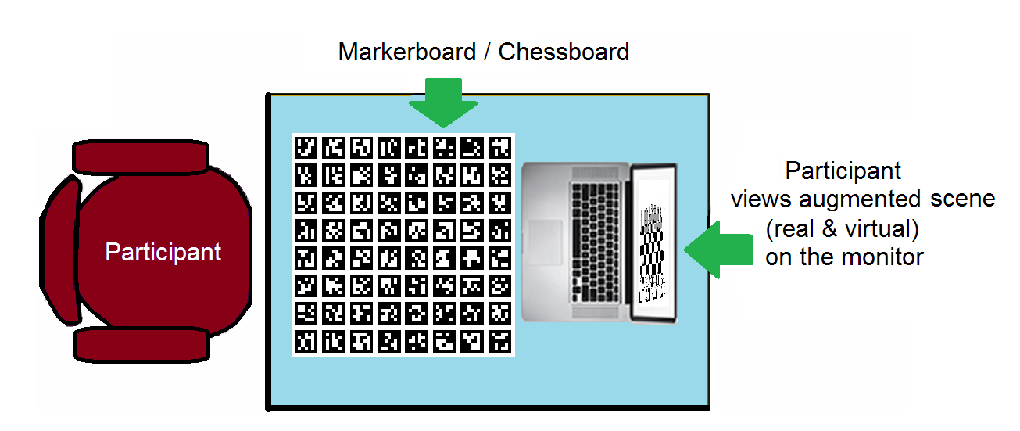
\includegraphics[scale=0.8, angle=0]{Files/Figures/planviewoftheexperimentalsetup.pdf}
    \caption[Κάτοψη της σχεδιασμού της πειραματικής εγκατάστασης]{Κάτοψη της σχεδιασμού της πειραματικής εγκατάστασης}
    \label{fig:plan_view}
\end{figure}


Η κάμερα RealSense\texttrademark{} 3D τοποθετείται στο πίσω μέρος ενός απλού καπέλου το οποίο φοράει ο χρήστης κατά τη διάρκεια των δοκιμών, εμπνευσμένο από παλαιότερη εργασία \cite{Mathews2007}. Όσο ο χρήστης φορά το καπέλο με τον αισθητήρα, ο αισθητήρας βλέπει προς το markerboard με αποτέλεσμα να "κοιτά" προς την περιοχή της αλληλεπίδρασης. Τέλος, ένας φορητός υπολογιστής τοποθετείται μπροστά από το markerboard και το χρήστη, ώστε να μπορεί να δει το επαυξημένο video που καταγράφει η κάμερα. Η κάμερα είναι συνδεδεμένη με το φορητό υπολογιστή, στον οποίο τρέχει η εφαρμογή. Η εικόνα~\ref{fig:test} δείχνει την πειραματική εγκατάσταση και έναν χρήστη κατά τη διάρκεια δοκιμής της εφαρμογής.



\begin{figure}[H]
\begin{subfigure}{.5\textwidth}
  \centering
  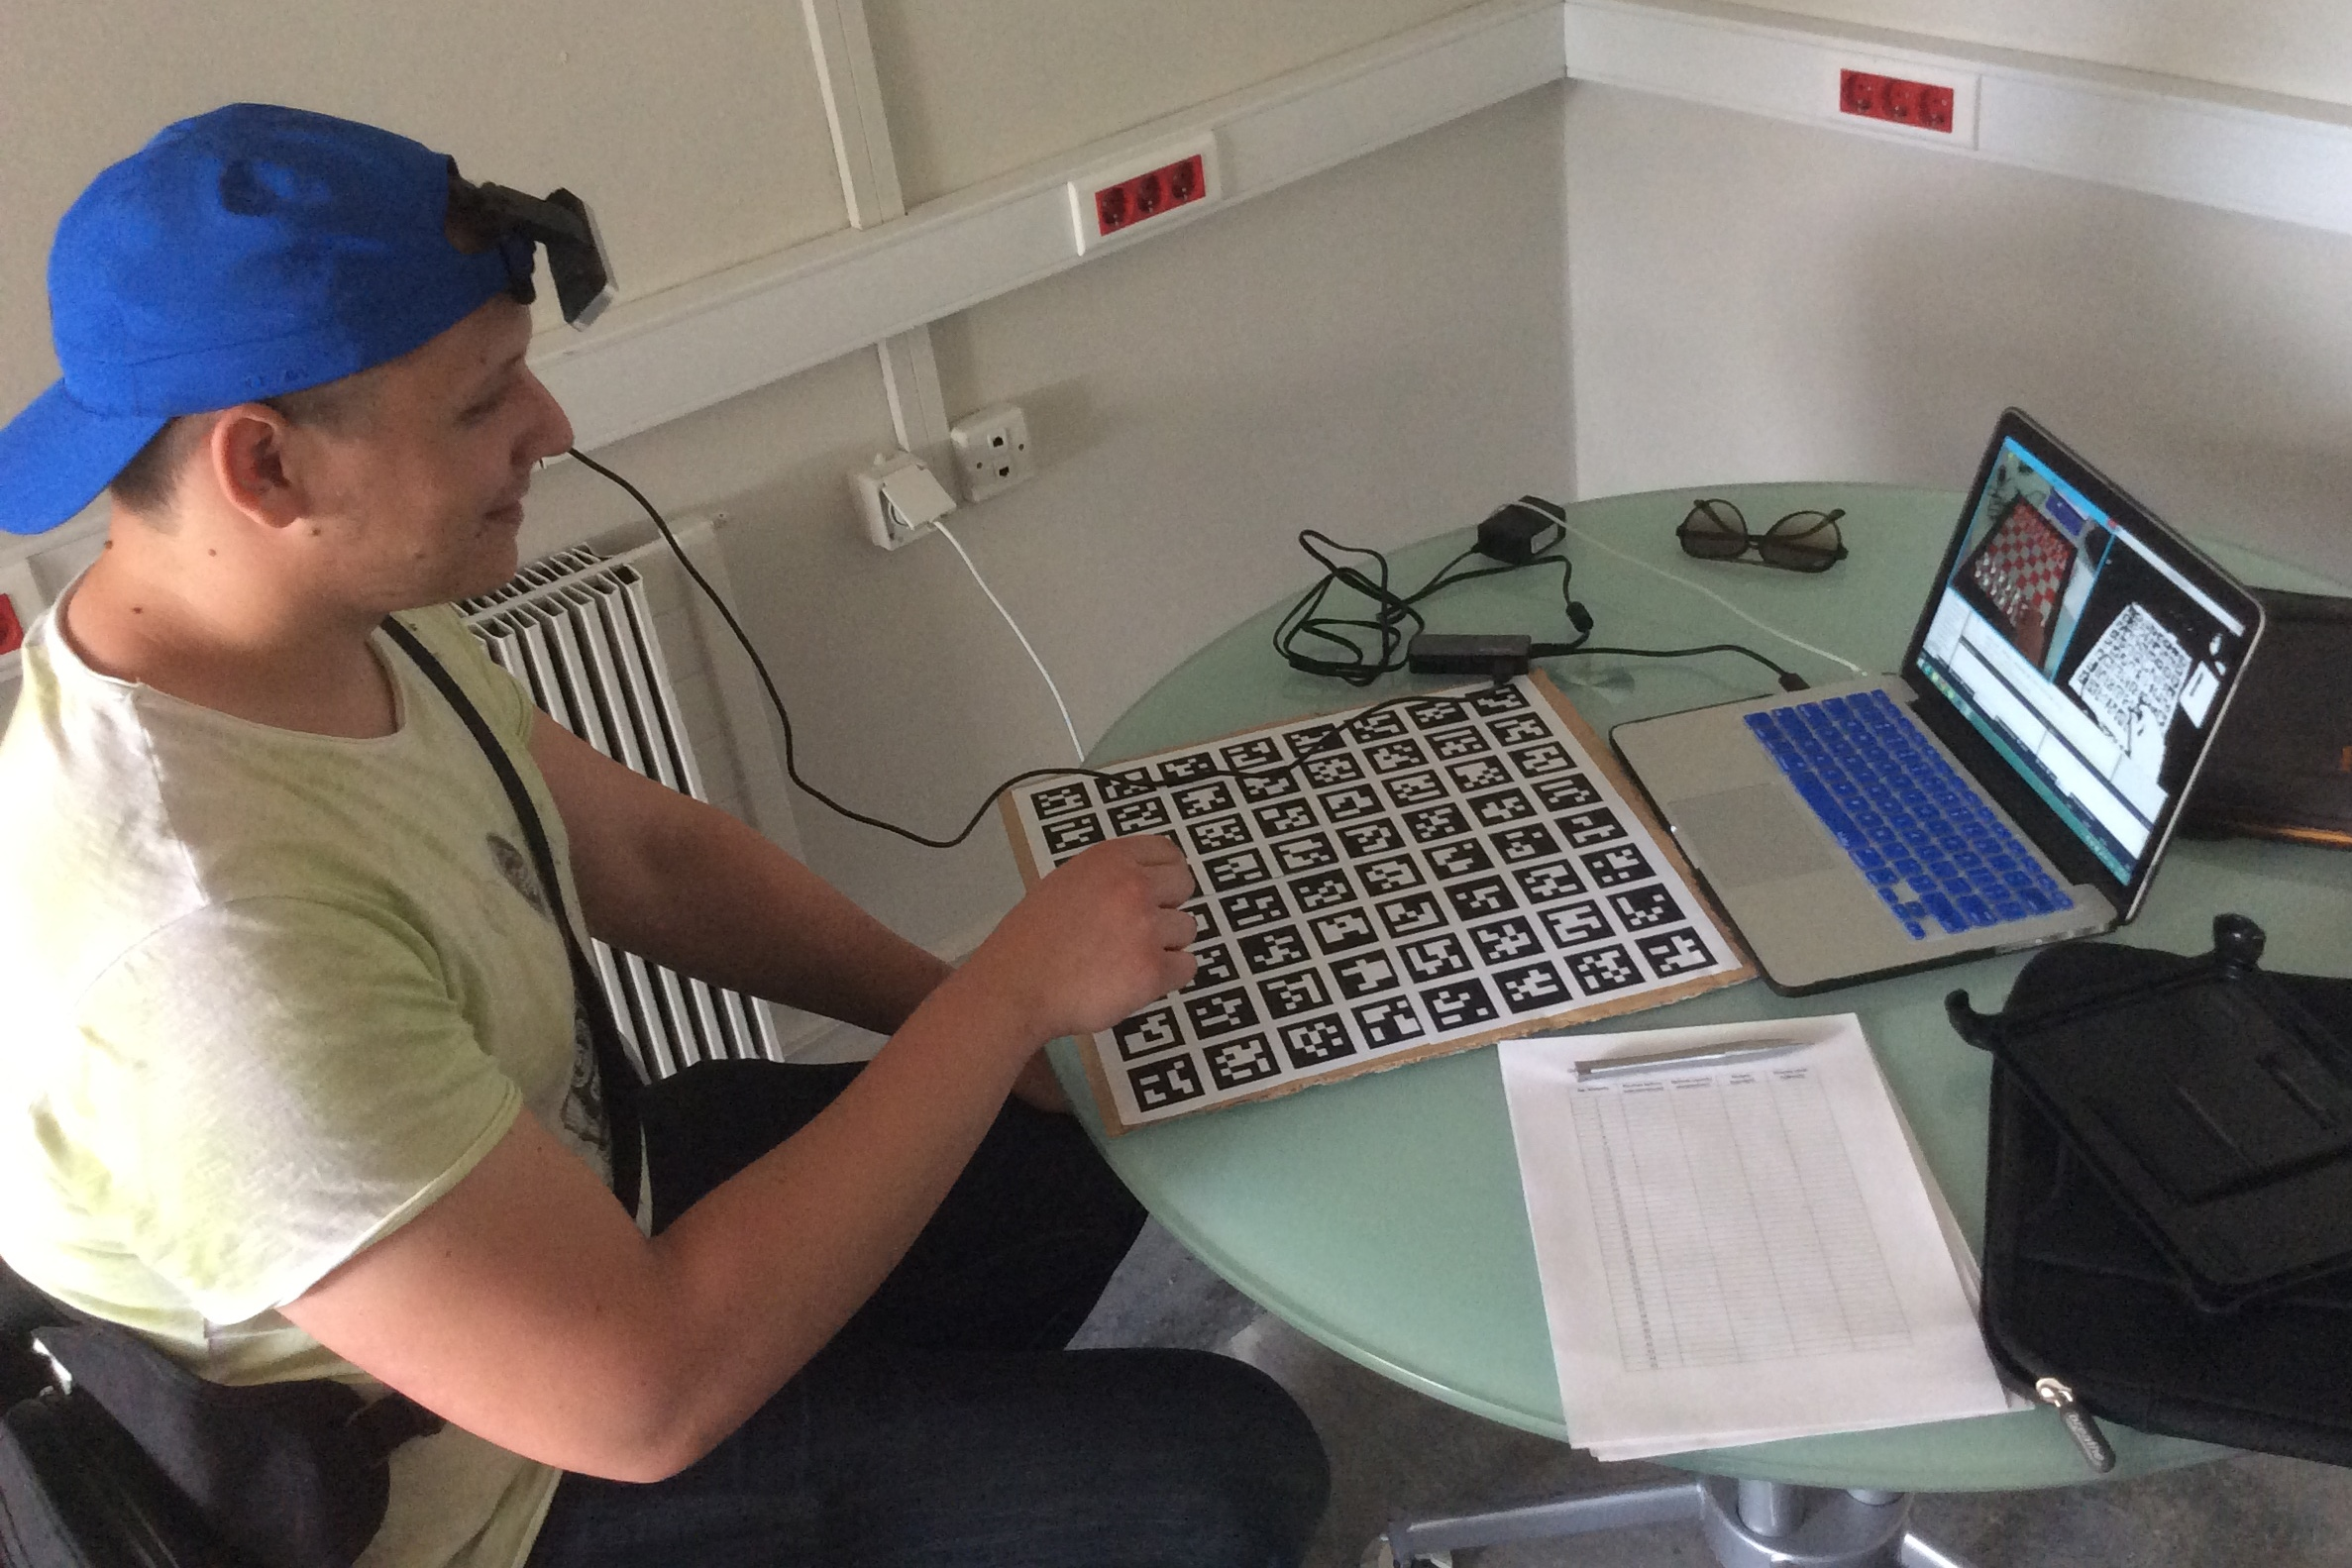
\includegraphics[width=.8\linewidth]{Files/Figures/user1.pdf}
  \caption{1a}
  \label{fig:sfiguser}
\end{subfigure}%
\begin{subfigure}{.5\textwidth}
  \centering
  \includegraphics[width=.7\linewidth]{Files/Figures/user2.pdf}
  \caption{1b}
  \label{fig:sfig2user}
\end{subfigure}\\
\caption{Φωτογραφία χρήστη κατά τη διάρκεια των δοκιμών}
\label{fig:test}
\end{figure}



\section{Βαθμονόμηση της Κάμερας}




Στα πλαίσια της διπλωματικής εργασίας απαιτείται η χρήση μιας απλής μεθόδου με αξιοποίηση συνηθισμένου εξοπλισμού για την βαθμονόμηση. Η διαδικασία της βαθμονόμησης απλοποιείται χρησιμοποιώντας ένα υπολογιστικό εργαλείο της OpenCV. 
Η διαδικασία περιλαμβάνει την καταγραφή ενός συνόλου φωτογραφιών ενός calibration board, και ο αλγόριθμος του εργαλείου υπολογίζει τις εσωτερικές παραμέτρους.
Το εργαλείο βαθμονόμησης αποθηκεύει τα αποτελέσματα σε ένα αρχείο, το οποίο διαβάζει η εφαρμογή επαυξημένης πραγματικότητας στην αρχή της εκτέλεσής της. 



%σκακιερα
Η OpenCV διαθέτει έτοιμες συναρτήσεις και εργαλεία για την βαθμονόμηση της κάμερας που βασίζονται σε μεθόδους που αναφέρθηκαν στο κεφάλαιο \ref{c:2}. Επιπλέον μέσω της OpenCV μπορούμε να μάθουμε τους συντελεστές παραμόρφωσης της κάμερας. 
Καταφεύγουμε λοιπόν, στη λύση του εργαλείου της Opencv για την βαθμονόμηση της κάμερας \cite{calibrationtool}, που προσφέρει μία έτοιμη και αποτελεσματική λύση, με χρήση μίας απλής κάμερας και μιας απλής επίπεδης εικόνας και συγκεκριμένα του μοτίβου τετραγώνων σκακιέρας, η οποία χρειάζεται απλά να εκτυπωθεί σε απλό χαρτί. 




Για τη διεξαγωγή της βαθμονόμησης απαιτείται η χρήση μιας απλής, επίπεδης εικόνας ασπρόμαυρης σκακιέρας, που μπορεί να εκτυπωθεί με ένα κοινό εκτυπωτή. Η διαδικασία αυτή είναι αυτόματη, ενώ τα μόνα δεδομένα εισόδου που θα πρέπει να δώσουμε στο εργαλείο της OpenCV είναι ο αριθμός των εσωτερικών γωνιών των τετραγώνων της. Για παράδειγμα το πρότυπο της βαθμονόμησης φαίνεται στο σχήμα~\ref{fig:pattern}, όπου έχουμε μία σκακιέρα, με αριθμό διαστάσεων με βάση τις εσωτερικές γωνίες 7x6. Η πληροφορία αυτή αξιοποιείται μέσω μεθόδων της OpenCV και επιστρέφονται ο πίνακας των εσωτερικών παραμέτρων της κάμερας και οι συντελεστές παραμόρφωσης. 


\begin{figure}[H]
\begin{subfigure}{.5\textwidth}
  \centering
  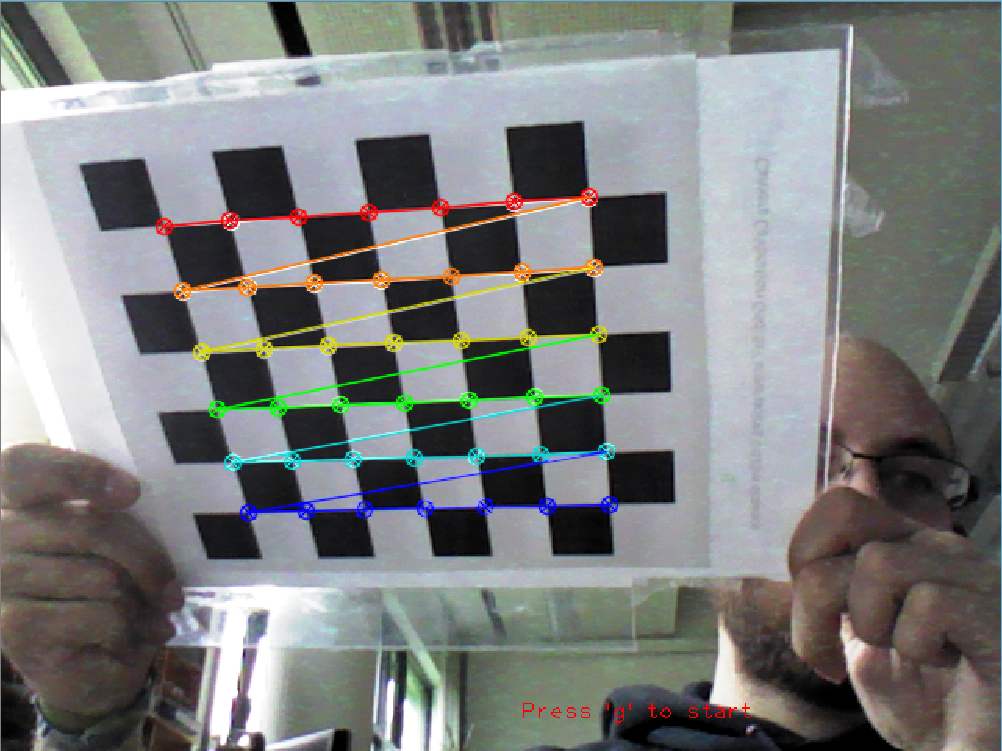
\includegraphics[width=.8\linewidth]{Files/Figures/calibration.pdf}
  \caption{1a}
  \label{fig:calibration_screenshot1}
\end{subfigure}%
\begin{subfigure}{.5\textwidth}
  \centering
  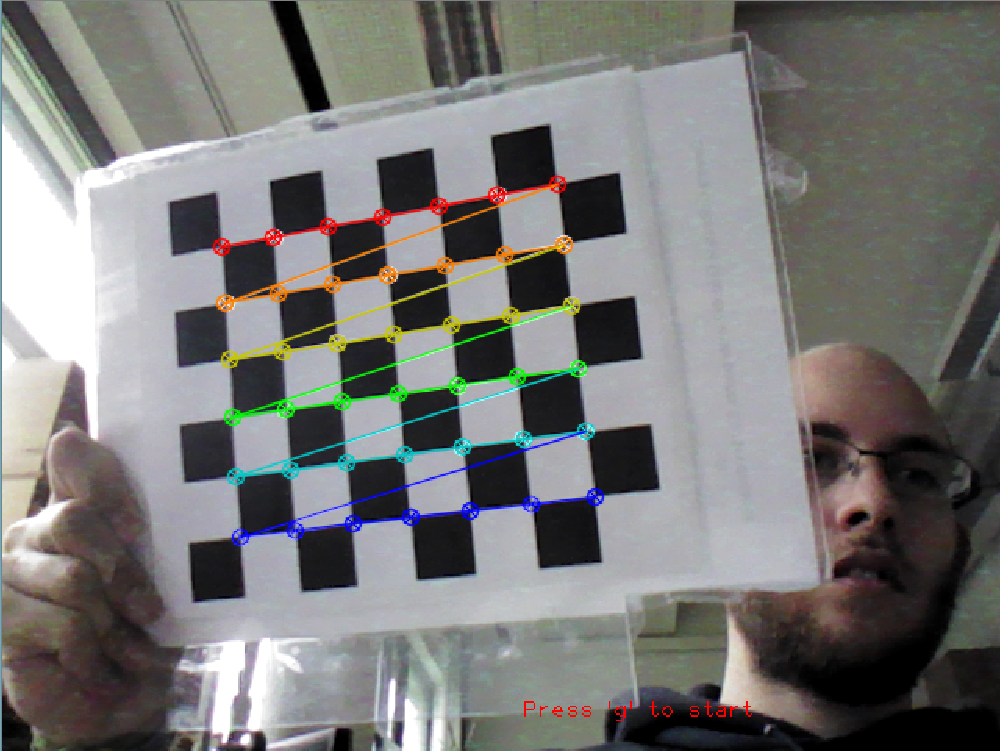
\includegraphics[width=.8\linewidth]{Files/Figures/calib2.pdf}
  \caption{1b}
  \label{fig:calibration_screenshot2}
\end{subfigure}
\caption[Στιγμιότυπο κατά τη διαδικασία της βαθμονόμησης κάμερας μέσω της OpenCV]{Στιγμιότυπο κατά τη διαδικασία της βαθμονόμησης κάμερας μέσω της OpenCV}
\label{fig:calibration_screenshot}
\end{figure}



Η βαθμονόμηση της κάμερας πραγματοποιείται μόνο μία φορά σαν αρχικό βήμα (offline calibration) κατά το αρχικό στάδιο της ανάπτυξης της εφαρμογής. Πιο συγκεκριμένα, κάνουμε ξεχωριστό calibration για κάθε διαφορετικό μοντέλο κάμερας που μπορεί να χρησιμοποιηθεί στην αναπτυσσόμενη εφαρμογή, καθώς και για κάθε διαφορετική ανάλυση αυτών. Το αποτέλεσμα είναι ένα ξεχωριστό αρχείο για κάθε κάμερα και κάθε ανάλυση που περιέχει τις αντίστοιχες εσωτερικές παράμετρους. Ανάλογα με τον εξοπλισμό και τις επιλογές του χρήστη φορτώνεται κατά την έναρξη της εφαρμογής το ανάλογο αρχείο. Έτσι οι εσωτερικές παράμετροι είναι γνωστές, ώστε σε μεταγενέστερο στάδιο να βρεθούν οι εξωτερικές παράμετροι.



\begin{figure}[H]
    \centering
    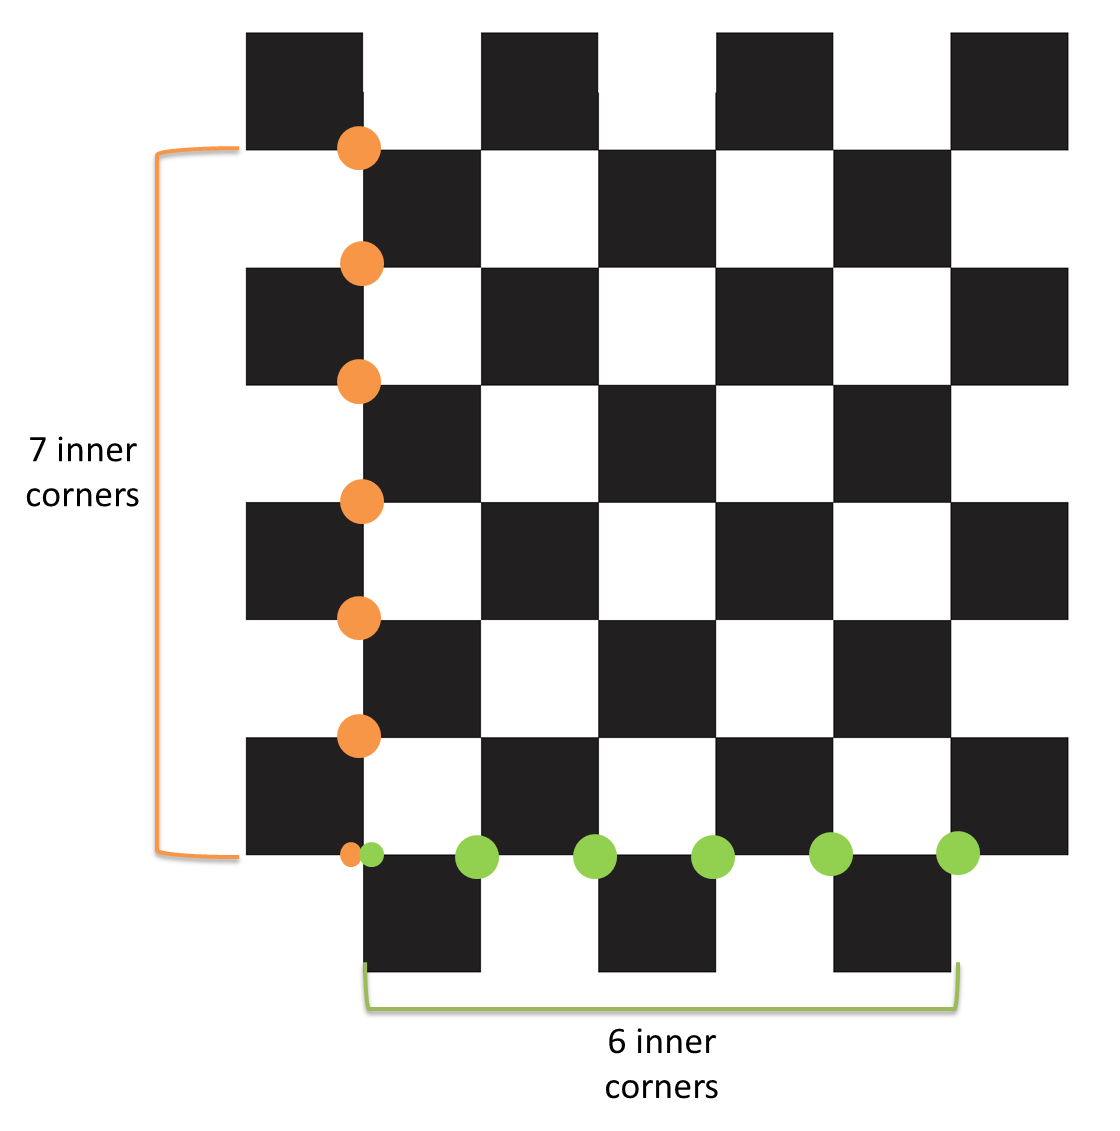
\includegraphics[scale=0.3, angle=0]{Files/Figures/pattern.pdf}
    \caption[Πρότυπο σκακιέρας για τη βαθμονόμησης της κάμερας]{Πρότυπο σκακιέρας για τη βαθμονόμησης της κάμερας}
    \label{fig:pattern}
\end{figure}




Στο πλαίσιο της παρούσας εργασίας, έγινε βαθμονόμηση με λήψη εικόνων επίπεδης σκακιέρας με μέγεθος 7 x 6 εσωτερικών γωνιών, με χρήση του παραδείγματος της βιβλιοθήκης OpenCV. Το μέγεθος κάθε τετραγώνου της σκακιέρας ορίστηκε στα 2,5cm. Το πρότυπο αυτό καταγράφηκε μέσω της κάμερας σε 25 διαφορετικές θέσεις. Η κάμερα διατηρήθηκε σε σταθερό σημείο και μετακινήσαμε την εκτυπωμένη εικόνα της σκακιέρας σε διαφορετικές θέσεις και με διαφορετικές κλίσεις. 






Η διαδικασία της βαθμονόμησης σε ανάλυση 640 x 480 έδωσε σαν αποτέλεσμα τις παρακάτω εσωτερικές παραμέτρους:


\begin{equation}
K=
\begin{bmatrix}
603.77848970443176 & 0 & 319.5\\
0 & 603.77848970443176 & 239.5\\
0 & 0 & 1
\end{bmatrix}
\end{equation}

Βλέποντας τις τιμές των principal points $c_{x}=319.5$ and $c{y}=239.5$ παρατηρούμε ότι είναι περίπου στο κέντρο των επιλεγμένων διαστάσεων δηλαδή κοντά στις τιμές  320 (640/2) και 240 (480/2). Επίσης βλέπουμε ότι $f_{x}=f_{y}$ που σημαίνει ότι χρησιμοποιείται κοινή εστιακή απόσταση και για τους 2 άξονες.


Εξ ορισμού η OpenCV μας δίνει 5 συντελεστές παραμόρφωσης, 3 ακτινικούς και 2 εφαπτομενικούς. Συγκεκριμένα κατά τη βαθμονόμηση πήραμε:

\begin{equation}
\begin{aligned}
k1= 0.16901284929874760\\
k2= -1.0214355567073656\\
p1= 0\\
p2= 0\\
k3= 1.3599972288823818 
\end{aligned}
\end{equation}

Το σφάλμα επαναπροβολής (Re-projection error) δίνει μία καλή εκτίμηση της ακρίβειας των παραμέτρων που βρέθηκαν κατά τη βαθμονόμηση της κάμερας. Η τιμή του πρέπει να είναι όσο γίνεται πιο κοντά στο 0 και υπολογίζεται με βάση τους πίνακες εσωτερικών παραμέτρων, συντελεστών παραμόρφωσης, περιστροφής και μετατόπισης. 


Μετά τη διαδικασία βαθμονόμησης το σφάλμα που πήραμε ήταν πολύ κοντά στο 0 και συγκεκριμένα :

\begin{equation}
Avg_{Reprojection_Error} = 0.20315774320090751
\end{equation}


\section{Δημιουργία Markerboard}


Ως επαύξηση της πραγματικότητας ορίζεται η διαδικασία πρόσθεσης εικονικής πληροφορίας σε εικόνες ή βίντεο. Για να συμβεί κάτι τέτοιο, πρέπει να γνωρίζουμε που ακριβώς πρέπει να απεικονιστεί η εικονική πληροφορία. Παρά το γεγονός ότι ορισμένες εφαρμογές αξιοποιούν τα φυσικά χαρακτηριστικά μιας σκηνής όπως η υφή ή σημεία κλειδιά, τα markers αποτελούν ακόμα έναν ελκυστικό τρόπο προσέγγισης επειδή είναι εύκολη η γρήγορη ανίχνευσή τους και η ακρίβεια που μπορεί να επιτευχθεί, όπως παρουσιάστηκε και στο~\ref{ssec:markerpose}. Μέσω της ανίχνευσης ενός marker όπως αυτοί που χρησιμοποιούνται από την ArUco μπορούν να υπολογιστούν οι εξωτερικές παράμετροι της κάμερας, δηλαδή η θέση και ο προσανατολισμός της σε σχέση με το marker ώστε να γνωρίζει το πρόγραμμα που πρέπει να σχεδιάσει τα 3D αντικείμενα και που είναι η αρχή των αξόνων (0,0,0) του συστήματος κοσμικών συντεταγμένων της σκηνής. 



Το γνωστό επιτραπέζιο παιχνίδι του σκακιού απαιτεί τη χρήση μιας σκακιέρας ως βάση προκειμένου να τοποθετηθούν τα πιόνια επάνω της. Kατά τη διάρκεια ενός παιχνιδιού σκακιού, ο χρήστης συχνά πρέπει να μετακινεί τα πιόνια με το χέρι του. Όταν συμβαίνει αυτό, το χέρι του χρήστη περνά πάνω από τη σκακιέρα αποκρύπτοντας ένα αρκετά σημαντικό μέρος της. 


Στα πλαίσια της παρούσας διπλωματικής εργασίας και προκειμένου να δημιουργήσουμε ένα σκάκι επαυξημένης πραγματικότητας θεωρήθηκε ότι η αξιοποίηση ενός markerboard προσομοιώνει τις ιδιότητες μιας σκακιέρας, ενώ η απόκρυψη μέρους του markerboard από το χέρι του χρήστη δεν επηρεάζει την απεικόνιση των εικονικών πιονιών κατά τη διάρκεια της μετακίνησης ενός πιονιού από το χρήστη. Επομένως αποφασίστηκε η δημιουργία ενός markerboard με μια διάταξη από 64 markers, σε ένα πλέγμα 8x8, με διαστάσεις ίδιες με αυτές μιας σκακιέρας. 


Οι δημιουργοί της βιβλιοθήκης ArUco δημοσίευσαν μία επιστημονική εργασία \cite{garrido2014automatic} όπου αναλύεται η μεθοδολογία για τη δημιουργία markerboard με markers τα στα οποία αντιστοιχίζονται συγκεκριμένα IDs με στόχο τον υψηλό αριθμό μεταβολών bits ώστε να μην μπερδεύονται τα markers με πραγματικά αντικείμενα του περιβάλλοντος, να ανιχνεύονται, δηλαδή, ευκολότερα από το σύστημα. 

Προτείνεται λοιπόν μια αυτόματη μέθοδος για την παραγωγή ενός markerboard με τον επιθυμητό αριθμό markers και τον επιθυμητό αριθμό bits. Χρησιμοποιώντας το έτοιμο εργαλείο που παρέχεται από τη βιβλιοθήκη ArUco για το σκοπό αυτό, δημιουργήσαμε μία "σκακιέρα" από markers υψηλής αξιοπιστίας, όπως φαίνεται και στην εικόνα~\ref{fig:markerboard}




\begin{figure}[H]
    \centering
    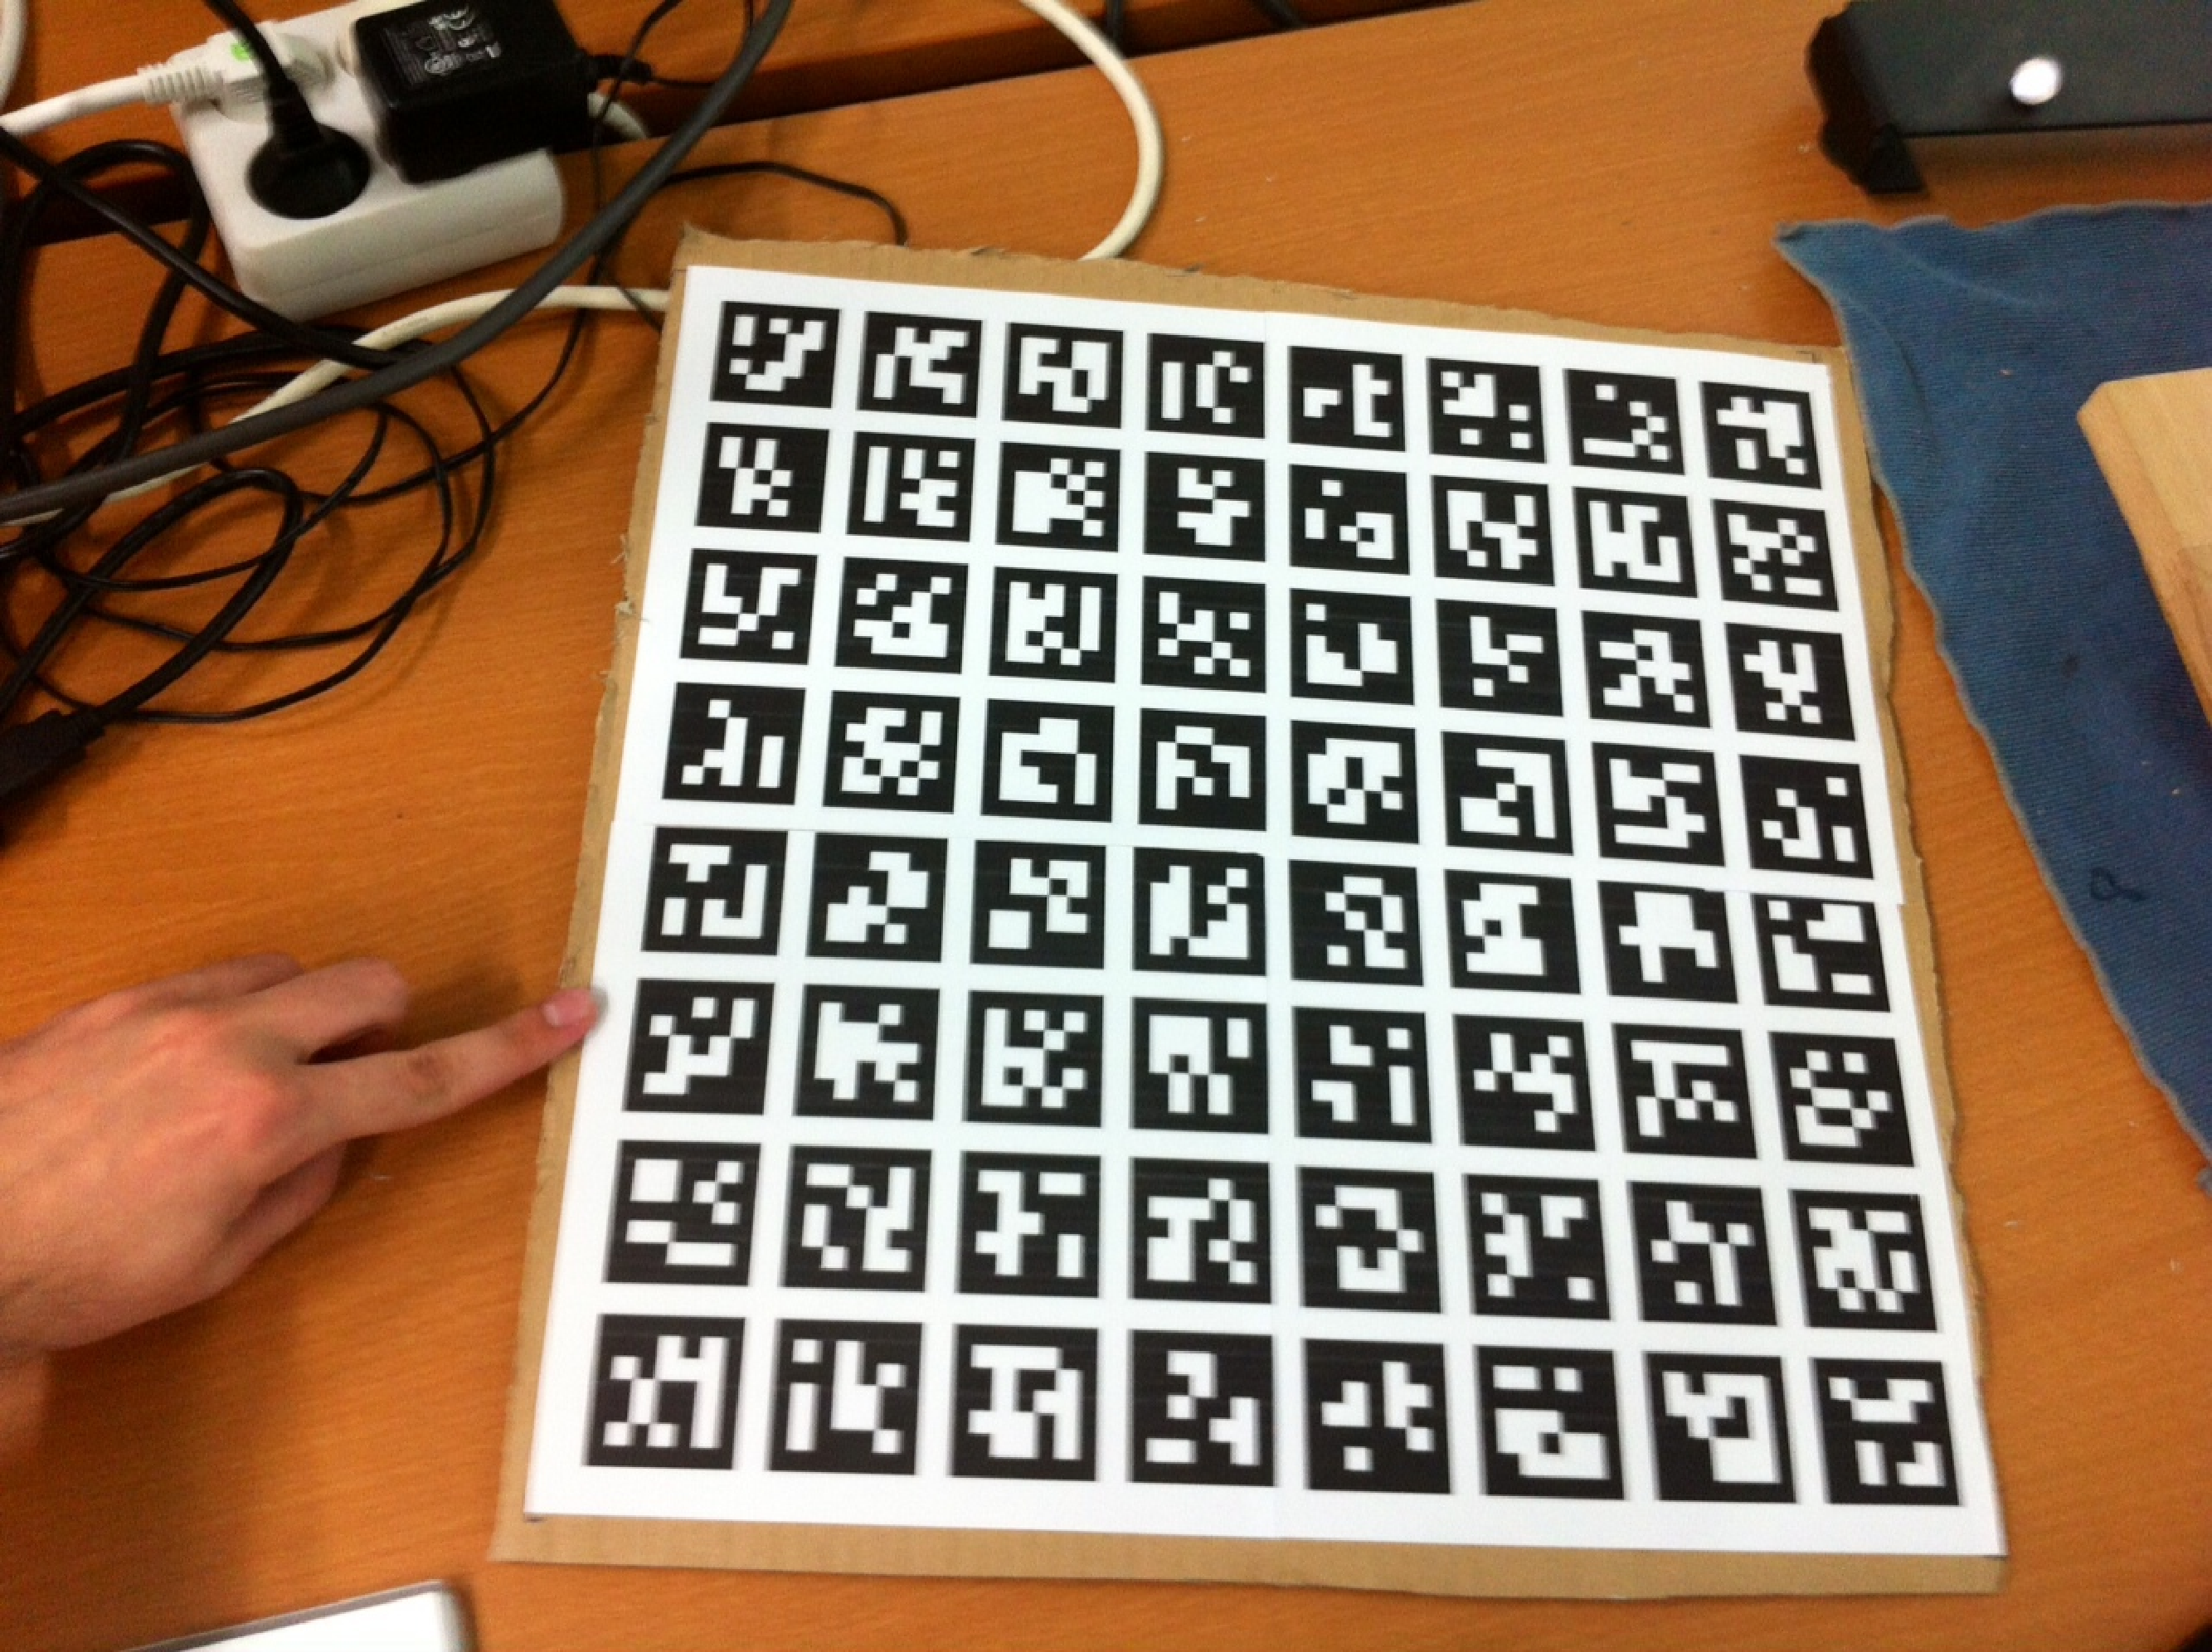
\includegraphics[width=0.5\textwidth]{Files/Figures/markerboard.pdf}
    \caption[Το markerboard που δημιουργήθηκε μέσω της ArUco]{Το markerboard που δημιουργήθηκε μέσω της ArUco}
    \label{fig:markerboard}
\end{figure}




\section{Ανίχνευση Θέσης Χειρονομίας "Τσιμπήματος"} \label{section:pinch}
%\section{Αναγνώριση Χειρονομίας Τσιμπήματος} 




Προκειμένου να ορίσουμε τον τρόπο με τον οποίο θα γίνεται ο εντοπισμός των χειρονομιών, καθώς και το είδος των χειρονομιών που πρέπει να ανιχνευτούν, χρειάζεται να καθοριστούν οι απαιτήσεις του συστήματος με λεπτομέρειες.
Για να αναπτυχθεί ένα σκάκι επαυξημένης πραγματικότητας, απαιτείται προφανώς αλληλεπίδραση σε πραγματικό χρόνο, σχετικά φθηνός εξοπλισμός και αλληλεπίδραση με όσο περισσότερο φυσικό τρόπο γίνεται, δηλαδή χωρίς τη χρήση ειδικών γαντιών ή καλωδίων. 

Οι απαιτήσεις του συστήματος για εκτέλεση των αλληλεπιδράσεων σε πραγματικό χρόνο, περιορίζει το επίπεδο της ανίχνευσης χειρονομιών που μπορεί να επιτευχθεί, ενώ παράλληλα οι απαιτήσεις για εξοπλισμό χαμηλού κόστους περιορίζουν την ποιότητα της εικόνας που πρέπει να καταγραφεί. Ο τρίτος περιορισμός που εισάγεται, προϋποθέτει τη χρήση τεχνικών όρασης υπολογιστών για την αναγνώριση των χειρονομιών του χρήστη, η απόδοση των οποίων περιορίζεται από τον επεξεργαστή του συστήματος. 



Η χειρονομία "τσιμπήματος" είναι μία χειρονομία που μπορεί να χρησιμοποιηθεί για την αλλεπίδραση με αντικείμενα στον τρισδιάστατο χώρο. Η χειρονομία "τσιμπήματος" μπορεί να πραγματοποιηθεί αρκετές φορές και υποδηλώνει φυσική κίνηση για επιλογή ενός αντικειμένου. Επομένως η αναγνώρισή της είναι βασική προϋπόθεση για την υλοποίηση βασικών αλληλεπιδράσεων με τα εικονικά αντικείμενα. 


Κατά τη διάρκεια της μετακίνησης ενός πιονιού στο σκάκι, μέρος του χεριού και των δακτύλων του χρήστη δεν είναι ορατά από την κάμερα. Για το λόγο αυτό, σκεφτήκαμε ότι η χρήση τεχνικών εντοπισμού της πόζας του χεριού μέσω ενός σκελετικού μοντέλου ή μέσω των μεθόδων που παρέχονται από το RealSense\texttrademark{} SDK θα ήταν υπερβολική για το συγκεκριμένο είδος εφαρμογής. Επομένως, δε χρειάζεται να ανιχνεύσουμε ούτε ολόκληρο το χέρι του χρήστη, ούτε τα δάκτυλα του αυτούσια. 



Με βάση τους παραπάνω περιορισμούς, η ανάπτυξη του συστήματος που αναπτύσσεται στην παρούσα διπλωματική εργασία, βασίστηκε στην εργασία του Andrew Wilson \cite{Wilson2006}, όπου παρουσιάζεται μία τεχνική υπολογιστικής όρασης για την εύκολη και γρήγορη αναγνώριση της κίνησης κατά την οποία ο αντίχειρας και ο δείκτης ενός χρήστη έρχονται κοντά (χειρονομία "τσιμπήματος") για εφαρμογές μικρής εμβέλειας και σχετικά ελεγχόμενες συνθήκες θέασης. Η τεχνική αυτή αποφεύγει πολύπλοκους και εύθραυστους αλγορίθμους εντοπισμού των χεριών, εντοπίζοντας την οπή που σχηματίζεται όταν ο δείκτης αγγίζει τον αντίχειρα του χρήστη. Το πρόβλημα της αλληλεπίδρασης μετατρέπεται ουσιαστικά σε πρόβλημα αναγνώρισης χειρονομιών. Περιγράφεται, δηλαδή, ένας εύκολος και γρήγορος τρόπος για την αναγνώριση της χειρονομίας τσιμπήματος. 


Συγκεκριμένα, υλοποιήθηκε ένα αλγόριθμος ανίχνευσης χειρονομιών, ο οποίος ενεργοποιεί μία εντολή αρπαγής και απελευθέρωσης των εικονικών πιονιών στην σκηνή της επαυξημένης πραγματικότητας. Χρησιμοποιούμε αυτή τη χειρονομία για να επιλέξουμε ένα πιόνι στη σκακιέρα και να μπορέσουμε να το μετακινήσουμε σε κάποια άλλη θέση.


Για να απλοποιηθεί αυτή η διαδικασία, πρέπει να οριστουν ορισμένες παραδοχές.
Πρώτα απ' όλα, το σύστημα θα πρέπει να χρησιμοποιείται με το δεξί χέρι του χρήστη, αν και μπορεί μελλοντικά να λυθεί αυτό το πρόβλημα εύκολα. Επιπλέον, η χειρονομία τσιμπήματος πρέπει να πραγματοποιείται με την ένωση του αντίχειρα και του δείκτη, αλλά και με τα υπόλοιπα δάκτυλα να είναι τεντωμένα και όσο γίνεται πιο κάθετα στο δείκτη, όπως φαίνεται στην εικόνα~\ref{fig:gesture_rec1}.

\begin{figure}[H]
    \centering
    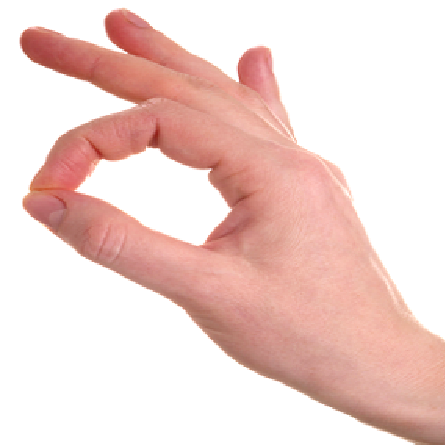
\includegraphics[scale=0.6, angle=0]{Files/Figures/correct_pinch.pdf}
    \caption[Παράδειγμα παραδοχής για τη σωστή χειρονομία "τσιμπήματος"]{Παράδειγμα παραδοχής για τη σωστή χειρονομία "τσιμπήματος"}
    \label{fig:gesture_rec1}
\end{figure}



Οι συναρτήσεις του SDK επιτρέπουν την ανίχνευση αντικειμένων μπροστά από την κάμερα, όπως είναι τα blobs και την εξαγωγή περιγραμμάτων και σημείων ενδιαφέροντος για αυτά τα blobs. Η ανίχνευση των blobs είναι μία εναλλακτική που βολεύει σε σχέση με τον εντοπισμό των χεριών που παρέχει το SDK, αφού η εφαρμογή μας δεν απαιτεί την ανίχνευση και τον εντοπισμό χεριών. Κάθε blob διαθέτει μία εξωτερική γραμμή περιγράμματος (contour line) και ανάλογα με στο σχήμα του blob, μία ή περισσότερες εσωτερικές γραμμές περιγράμματος. Κάθε τέτοια γραμμή περιγράμματος αναπαρίσταται από μία σειρά σημείων. Οι εξωτερικές γραμμές περιγραμμάτων (εξωτερικά σύνορα), καθώς και οι εσωτερικές γραμμές των περιγραμμάτων ορίζονται από ένα πίνακα σημείων.


Η προσέγγιση μας, αξιοποιεί τα δεδομένα των blobs και την οπή που σχηματίζεται όταν ο αντίχειρας ακουμπά ή βρίσκεται πολύ κοντά στον δείκτη. Πιο συγκεκριμένα, υλοποιήθηκε ένας αλγόριθμος που ανιχνεύει πότε λαμβάνει χώρα μία χειρονομία τσιμπήματος και που ακριβώς στον 3D χώρο. Γνωρίζοντας το σημείο στο 3D χώρο στο οποίο συμβαίνει η χειρονομία, μπορούμε να επιλέξουμε το σωστό πιόνι και να το μετακινήσουμε ανάλογα. 


Η απρόσκοπτη ανίχνευση μιας χειρονομίας τσιμπήματος είναι η βάση για τη σωστή λειτουργία του συστήματός μας και για αυτό το λόγο θα αναφερθούμε ξεχωριστά στην αναγνώριση και την ανίχνευση της θέσης στην οποία πραγματοποιείται η χειρονομία. Ο αλγόριθμος που σχεδιάστηκε αναλύεται στη συνέχεια.



Σε κάθε frame, παίρνουμε τις εικόνες βάθους και χρώματος που καταγράφει η συσκευή. Λόγω της λανθασμένης ευθυγράμμισης και της φυσικής απόκλισης της θέσης του αισθητήρα χρώματος σε σχέση με τον αισθητήρα βάθους (αφού δεν βρίσκονται ο ένας πάνω στον άλλο), χρειάζεται ένας τρόπος να αντιστοιχηθούν τα εικονοστoιχεία χρώματος με τα εικονοστοιχεία βάθους και αντίστροφα. Για το συγκεκριμένο λόγο, η βιβλιοθήκη RealSense παρέχει μία δομή με το όνομα UVMap η οποία επιτελεί αυτό το συγκεκριμένο σκοπό.

Στην αρχή της διαδικασίας, χρειάζεται να χρησιμοποιήσουμε τις ιδιότητες της βιβλιοθήκης για εξαγωγή των blobs. Πριν συμβεί αυτό, πρέπει να ορίσουμε κάποιες παραμέτρους, όπως τον μέγιστο αριθμό blobs που θέλουμε να ανιχνευτούν και το επίπεδο της εξομάλυνσης κατά την κατάτμηση της εικόνας για να πάρουμε τα σωστά περιγράμματα του blob. 

Στην προσέγγιση μας, επιλέξαμε να ανιχνεύεται το κοντινότερο blob της εικόνας βάθους ως προς την κάμερα, διότι κατά τη διάρκεια ενός παιχνιδιού σκακιού ως προς το σημείο παρατήρησης του χρήστη (π.χ τα μάτια του), το ρόλο αυτό παίζουν τα χέρια του, τα οποία και όντως θέλουμε να εντοπίσουμε. Μόλις αναγνωριστεί το κοντινότερο blob, ωστόσο, πρέπει να το επεξεργαστούμε για να δούμε αν όντως πρόκειται για ένα blob χεριού ή για κάποιο άλλο αντικείμενο.


\begin{figure}[H]
    \centering
    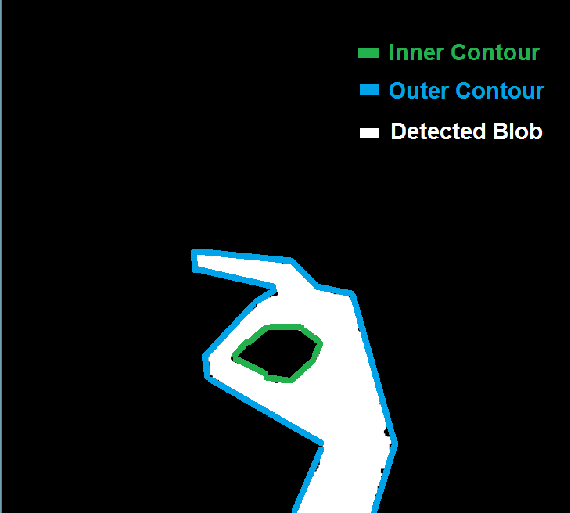
\includegraphics[scale=0.7, angle=0]{Files/Figures/2.pdf}
    \caption[Παράδειγμα blob χεριού και περιγραμμάτων που σχηματίζονται]{Παράδειγμα blob χεριού και περιγραμμάτων που σχηματίζονται}
    \label{fig:hand_blob}
\end{figure}



Για το λόγο αυτό, παίρνουμε μέσω του SDK τον αριθμό των περιγραμμάτων που ανιχνεύθηκαν στο συγκεκριμένο blob. Αν ο αριθμός αυτός είναι μικρότερος του 2, αυτόματα συνεπάγεται ότι δεν υπάρχουν εσωτερικά περιγράμματα και επομένως δεν υπάρχει οπή στην εικόνα μας. Έτσι το πρόγραμμα γνωρίζει σίγουρα ότι ο χρήστης δεν εκτέλεσε χειρονομία "τσιμπήματος". Από την άλλη πλευρά, αν ο αριθμός των περιγραμμάτων είναι μεγαλύτερος του 2, τότε είναι πιθανό να έλαβε χώρα μια χειρονομία τσιμπήματος. 


Για να ελέγξουμε αν συνέβη κάτι τέτοιο, παίρνουμε τον αριθμό των σημείων που απαρτίζουν το εσωτερικό περίγραμμα που ανιχνεύθηκε. Αν ο αριθμός των σημείων αυτών είναι μικρότερος από ένα κατώφλι, δηλαδή μία τιμή που ορίζεται μέσω δοκιμών, τότε μπορούμε είτε να συμπεράνουμε ότι τα δεδομένα του περιγράμματος δε σχετίζονται με το χέρι του χρήστη, είτε ότι το χέρι είναι πολύ μακριά από την κάμερα, και μπορούμε να συνεχίσουμε την ανάλυση του επόμενου frame. Αν όμως ο αριθμός των σημείων είναι μεγαλύτερος της τιμής κατωφλίου που ορίστηκε, τότε μπορούμε να αποφανθούμε ότι έχουμε μία χειρονομία "τσιμπήματος". Όταν συμβεί κάτι τέτοιο πρέπει να ελέγξουμε τη θέση στην οποία συνέβη η χειρονομία στο 3D χώρο. Η διαδικασία αυτή περιγράφεται στην επόμενη ενότητα, ενώ ο αλγόριθμος αναγνώρισης χειρονομίας "τσιμπήματος" που περιγράφηκε φαίνεται στο σχήμα~\ref{fig:gesture_rec}.







\begin{figure}[H]
    \centering
    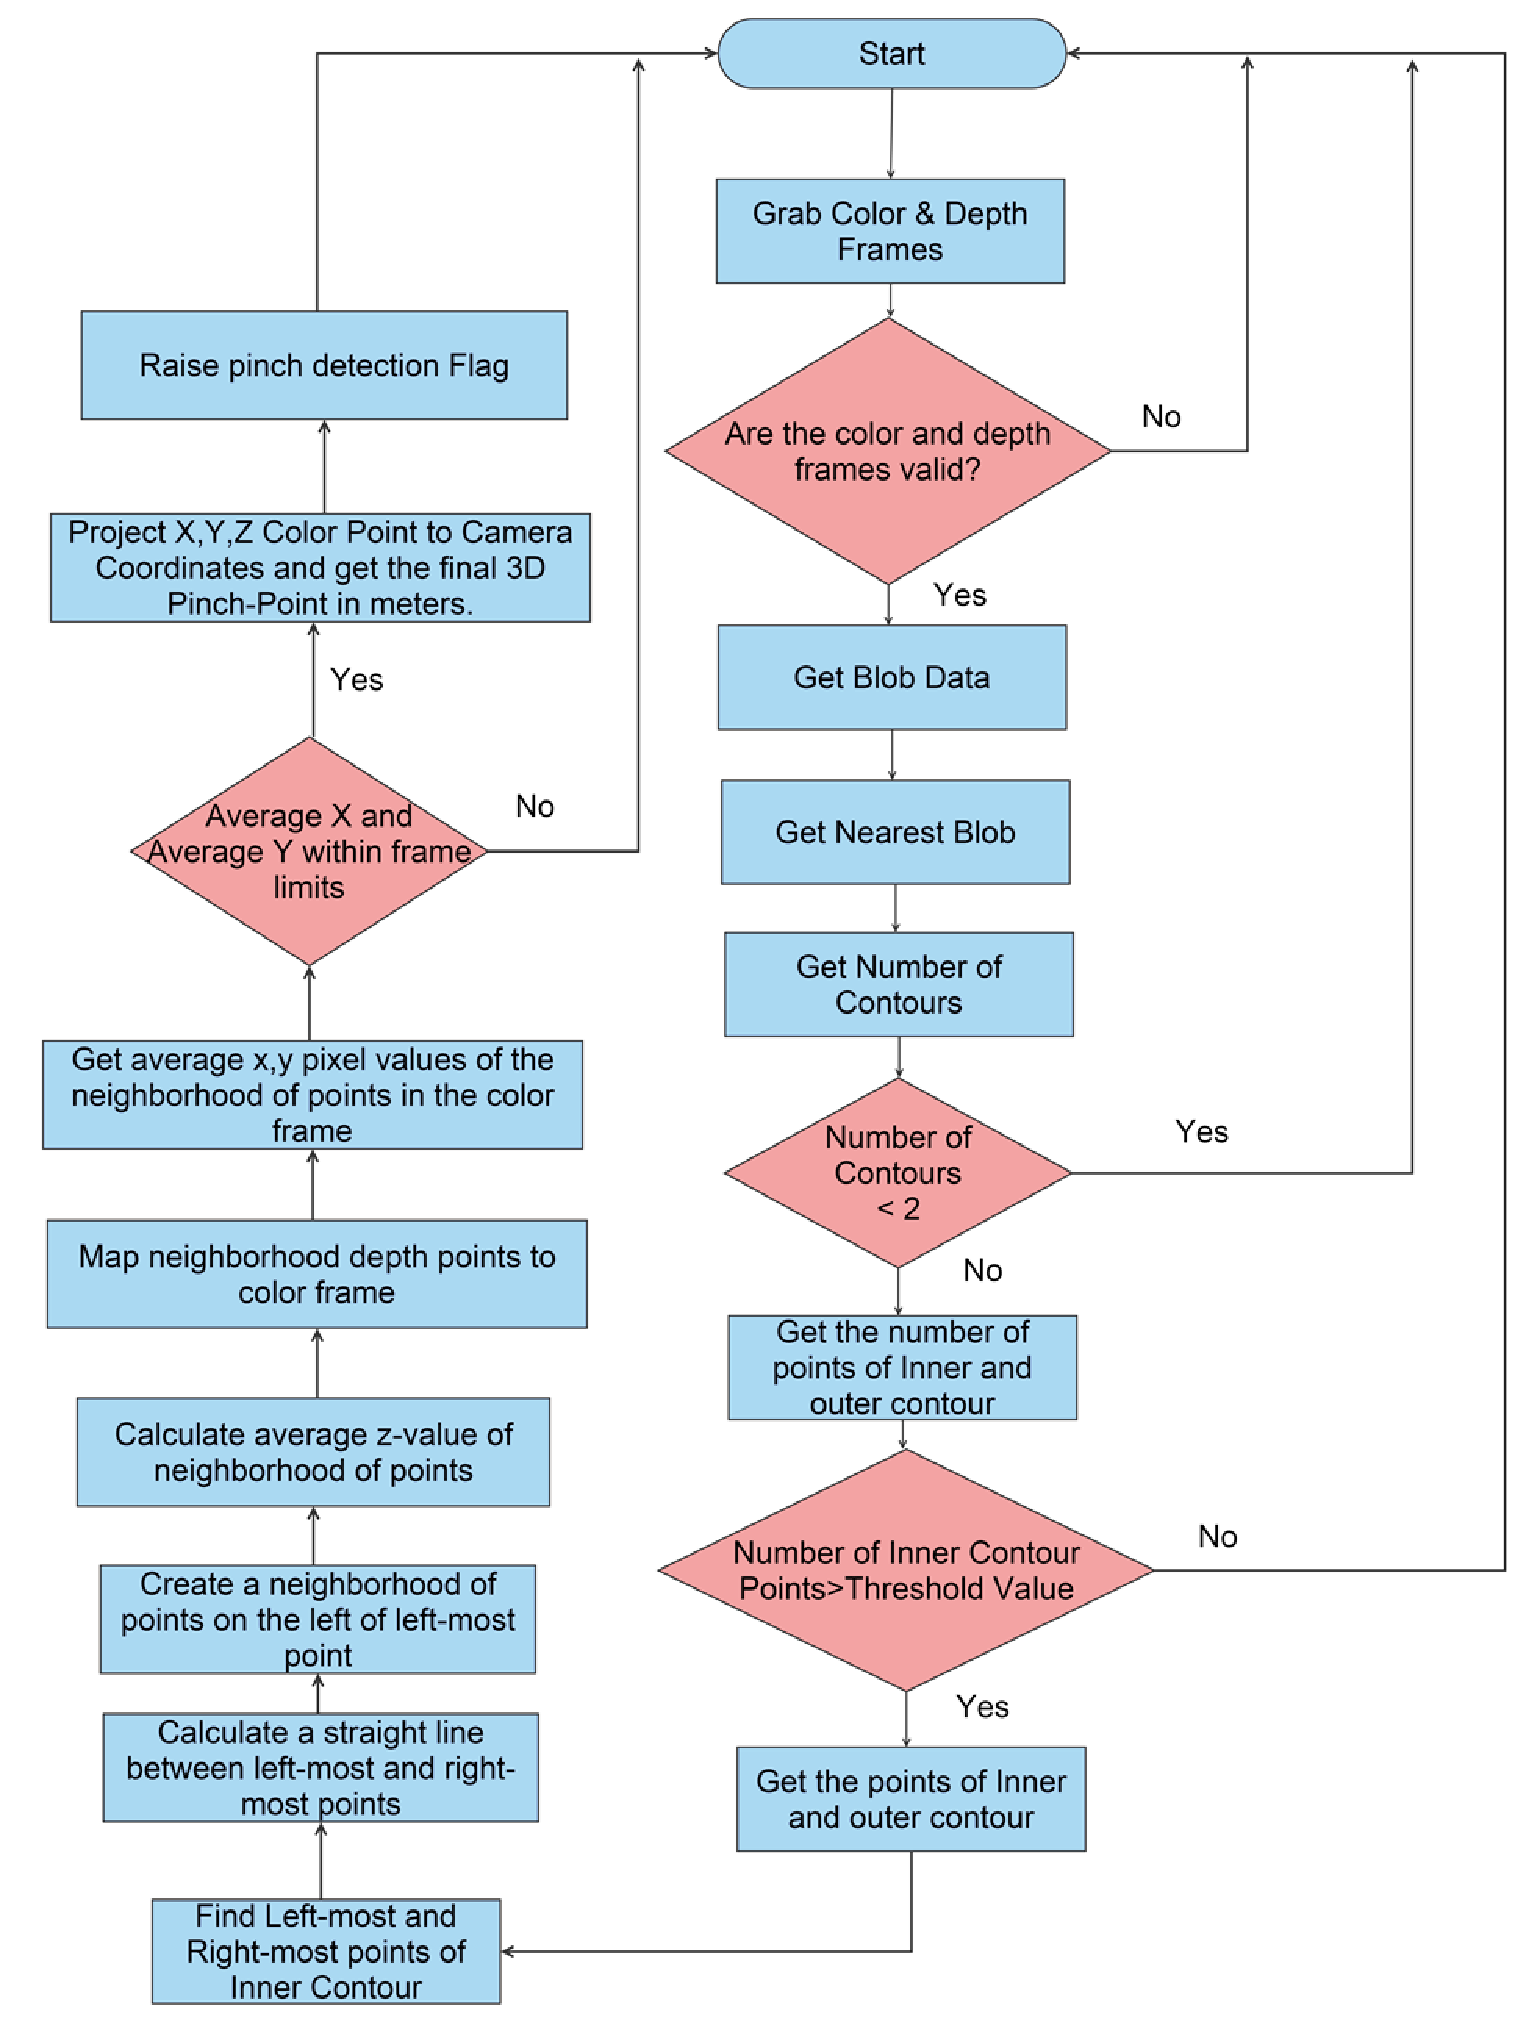
\includegraphics[width=.85\linewidth]{Files/Figures/pinch_gesture_detection.pdf}
    \caption[Διάγραμμα του αλγορίθμου ανίχνευσης χειρονομίας "τσιμπήματος"]{Διάγραμμα του αλγορίθμου ανίχνευσης χειρονομίας "τσιμπήματος"}
    \label{fig:gesture_rec}
\end{figure}



\begin{figure}[H]
    \centering
    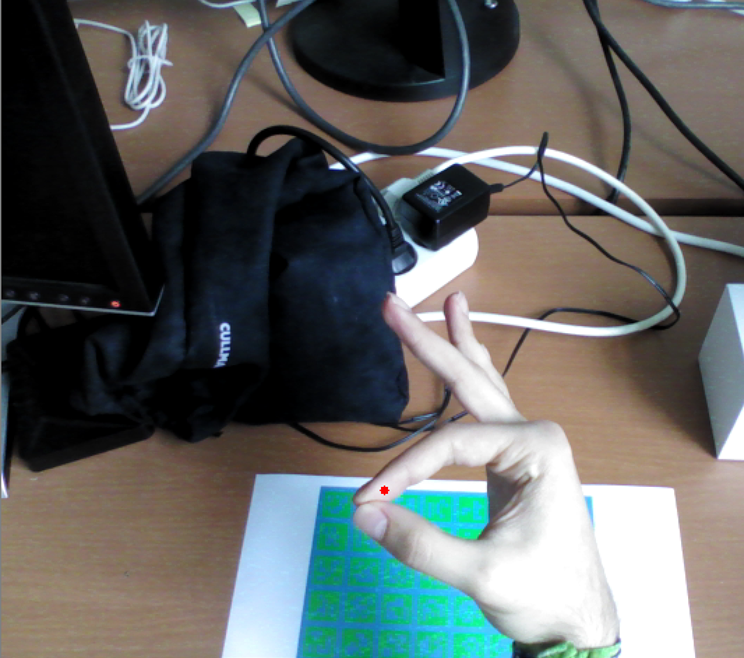
\includegraphics[width=0.45\textwidth]{Files/Figures/pinch.png}
    \caption[Στιγμιότυπο αποτελέσματος αναγνώρισης χειρονομίας "τσιμπήματος"]{Στιγμιότυπο αποτελέσματος αναγνώρισης χειρονομίας "τσιμπήματος"}
    \label{fig:pinch results}
\end{figure}







Μία σημαντική συνεισφορά της παρούσας διπλωματικής εργασίας αφορά τη μεθοδολογία που παρουσιάζεται σε αυτή την ενότητα, σχετικά με τον εντοπισμό της θέσης όπου λαμβάνει χώρα μία χειρονομία "τσιμπήματος" για συστήματα αλληλεπίδρασης επαυξημένης πραγματικότητας. Στόχος μας είναι να δημιουργηθεί ένα σύστημα αναγνώρισης χειρονομιών για την τρισδιάστατη αλληλεπίδραση και το χειρισμό των εικονικών αντικειμένων. Κάτι τέτοιο πραγματοποιείται χωρίς να χρειάζονται πολύπλοκες διαδικασίες ανάλυσης της κίνησης των δακτύλων ή του χεριού. Αντίθετα, αξιοποιούνται απλές τεχνικές επεξεργασίας εικόνας και υπολογιστικής όρασης.


Στην προηγούμενη ενότητα, παρουσιάστηκε ένας τρόπος ανίχνευσης της χειρονομίας "τσιμπήματος", ωστόσο αυτό μόνο δεν αρκεί για την μετακίνηση των πιονιών του σκακιού στην εφαρμογή που θέλουμε να αναπτύξουμε. Πρέπει να βρούμε το σημείο στο οποίο συνέβη η χειρονομία στο 3D χώρο, με όσο μεγαλύτερη ακρίβεια γίνεται. 



Αν κατά το στάδιο της ανίχνευσης μιας χειρονομίας "τσιμπήματος" διαπιστώθεί ότι έχουμε όντως μία τέτοια χειρονομία, δηλαδή ο αριθμός των περιγραμμάτων του blob είναι μεγαλύτερος ή ίσος του 2 και ο αριθμός των σημείων του εσωτερικού περιγράμματος είναι μεγαλύτερος από μία τιμή κατωφλίου, μπορούμε να συνεχίσουμε για να βρούμε τη θέση στην οποία πραγματοποιήθηκε η χειρονομία ως προς την κάμερα.

Για να συμβεί αυτό, αρχικά επιλέγεται το σημείο του εσωτερικού περιγράμματος που βρίσκεται όσο γίνεται πιο αριστερά, όσον αφορά την εικόνα blob, καθώς και το σημείο του εσωτερικού περιγράμματος που βρίσκεται όσο γίνεται πιο δεξιά. Με βάση αυτά τα 2 σημεία, μπορούμε να βρούμε μία μοναδική ευθεία που ορίζεται από αυτά. Στη συνέχεια, μπορούμε να δημιουργήσουμε μία περιοχή ή καλύτερα μία "γειτονιά"  ενός παραμετρικού αριθμού σημείων, που ανήκουν στη συγκεκριμένη ευθεία που υπολογίστηκε και βρίσκονται αριστερά από το πιο αριστερό σημείο του εσωτερικού περιγράμματος.  Ο αριθμός των σημείων που μπορούμε να πάρουμε μπορεί να οριστεί ως παράμετρος στο πρόγραμμά μας. Προφανώς, όσο περισσότερα σημεία επιλέξουμε, τόσο πιο ακριβές θα είναι το αποτέλεσμα, αλλά τόσο πιο αργό θα γίνεται το πρόγραμμα όπως θα διαπιστωθεί στη συνέχεια. 


Μόλις εκτιμηθεί αυτή η "γειτονιά" σημείων στο frame της εικόνας , μπορούμε να υπολογίσουμε τις τιμές βάθους για καθένα από αυτά τα σημεία και επομένως να εκτιμήσουμε τη μέση τιμή βάθους των εικονοστοιχείων της "γειτονιάς" τα οποία έχουν έγκυρες τιμές. Αυτή η μέση τιμή βάθους, μπορεί να χρησιμποιηθεί αργότερα ως η τιμή βάθους στην οποία πραγματοποιείται η χειρονομία "τσιμπήματος" στον τρισδιάστατο χώρο της σκηνής. 

Αξιοποιώντας, τη δομή UVMap, στην οποία αναφερθήκαμε στην οποια αναφερθήκαμε προηγουμένως, μπορούμε να αντιστοιχίσουμε κάθε σημείο, δηλαδή κάθε εικονοστοιχείο της "γειτονιάς" σημείων στην εικόνα χρώματος που καταγράφει ο αισθητήρας στο ίδιο frame. Υπολογίζουμε τη μέση τιμή των συντεταγμένων εικόνας στην οποία βρίσκεται κάθε σημείο και έχει έγκυρες τιμές (αφού κατά την αντιστοίχιση μπορεί να έχουμε λανθασμένες προσεγγίσεις). Ωστόσο οι τιμές αυτές μετρώνται σε pixels ενώ εμείς θέλουμε να βρούμε το σημείο στο οποίο έλαβε χώρα η χειρονομία στο 3D χώρο σε μονάδες του πραγματικού κόσμου (π.χ μέτρα). Επομένως, πρέπει να προβάλλουμε αυτά τα εικονοστοιχεία χρώματος στο σύστημα συντεταγμένων της κάμερας ώστε να πάρουμε τις αποστάσεις σε μονάδες του πραγματικού κόσμου, δηλαδή στην περίπτωσή μας σε μέτρα. Κάτι τέτοιο μπορεί να γίνει εύκολα μέσω του RealSense SDK.


Μόλις ολοκληρωθεί αυτή η διαδικασία, έχουμε τις τιμές των συντεταγμένων $x,y,z$ για ένα συγκεκριμένο σημείο στον τρισδιάστατο χώρο σε μέτρα, το οποίο θεωρούμε ως το σημείο στο οποίο πραγματοποιήθηκε η χειρονομία "τσιμπήματος" από το χρήστη, ή αλλιώς ως το σημείο στον τρισδιάστατο χώρο όπου ο χρήστης αποφάσισε να "τσιμπήσει" κάποιο εικονικό αντικείμενο. Προφανώς, μόλις συμβεί κάτι τέτοιο και αν οι συντεταγμένες έχουν μία έγκυρη τιμή, ενεργοποιείται μία σημεία που υποδηλώνει στο πρόγραμμά μας ότι πραγματοποιήθηκε μία χειρονομία "τσιμπήματος". 

Εν τέλει, έχουμε το σημείο "τσιμπήματος" στον τρισδιάστατο χώρο ως προς τον αισθητήρα χρώματος της συσκευής. Με βάση την μεθοδολογία που αναφέρθηκε, μπορούμε να αναπτύξουμε την εφαρμογή μας και να υλοποιήσουμε τη λογική του βιντεοπαιχνιδιού σκακιού επαυξημένης πραγματικότητας. 




\begin{figure}[H]
\begin{subfigure}{.5\textwidth}
  \centering
  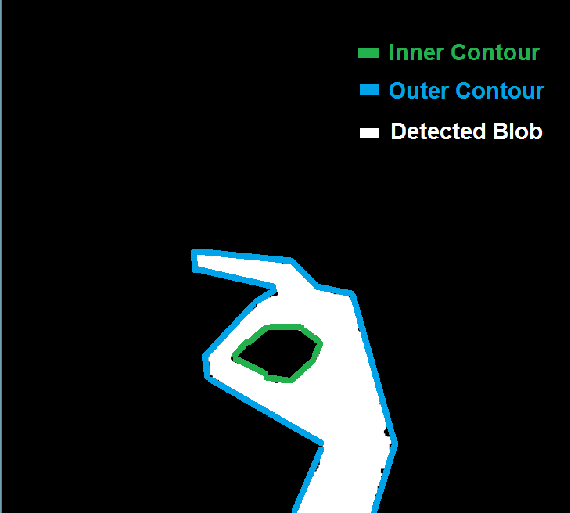
\includegraphics[width=.8\linewidth]{Files/Figures/2.pdf}
  \caption{1a}
  \label{fig:sfig11}
\end{subfigure}%
\begin{subfigure}{.5\textwidth}
  \centering
  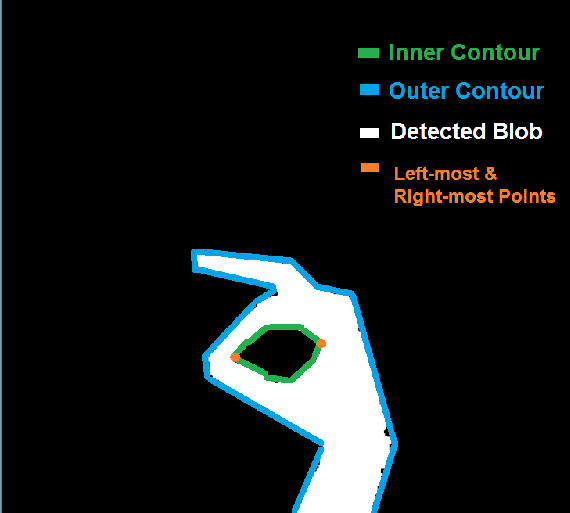
\includegraphics[width=.8\linewidth]{Files/Figures/3.pdf}
  \caption{1b}
  \label{fig:sfig22}
\end{subfigure}\\
\begin{subfigure}{.5\textwidth}
  \centering
  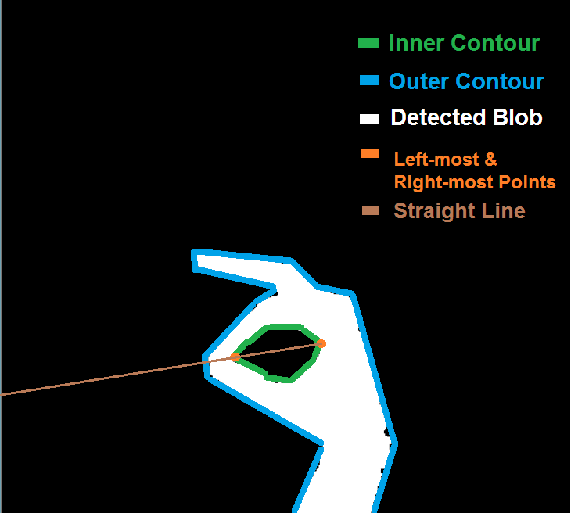
\includegraphics[width=.8\linewidth]{Files/Figures/4.pdf}
  \caption{1a}
  \label{fig:sfig111}
\end{subfigure}%
\begin{subfigure}{.5\textwidth}
  \centering
  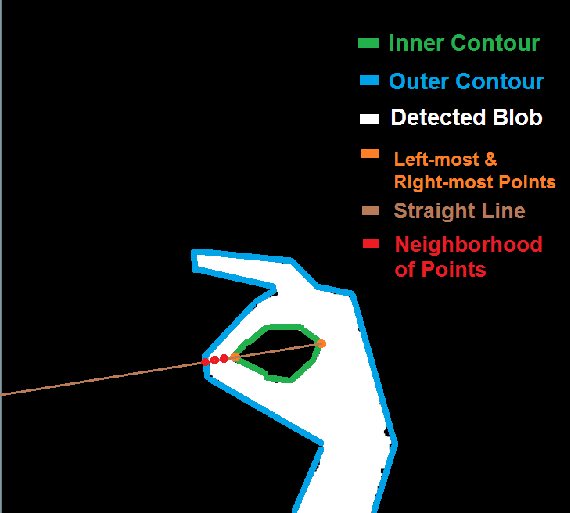
\includegraphics[width=.8\linewidth]{Files/Figures/5.pdf}
  \caption{1b}
  \label{fig:sfig2222}
\end{subfigure}
\caption{Φάσεις εντοπισμού χειρονομίας "τσιμπήματος" στο χώρο}
\label{fig:fig}
\end{figure}



Αφού όλα τα εικονικά αντικείμενα απεικονίζονται ως προς την αρχή των συντεταγμένων του κέντρου της σκακιέρας, δηλαδή του markerboard, η αλληλεπίδραση ανάμεσα στα πραγματικά και τα εικονικά αντικείμενα θα πρέπει να πραγματοποιείται ως προς αυτό το κοινό σύστημα συντεταγμένων. Επομένως, στην επόμενη ενότητα θα παρουσιαστεί η διαδικασία μετατροπής του 3D σημείου όπου πραγματοποιήθηκε η χειρονομία "τσιμπήματος", από το σύστημα συντεταγμένων κάμερας στο σύστημα συντεταγμένων του markerboard.



\section{Tαυτοποίηση Συστημάτων Συντεταγμένων}



Ο μηχανισμός αλληλεπίδρασης που παρουσιάστηκε στις προηγούμενες ενότητες αφορά τη μοντελοποίηση ενός τρόπου επιλογής και χειρισμού εικονικών αντικειμένων που θα μπορούσε κάποιος να παρομοιάσει με το κλικάρισμα ενός ποντικιού και τη μετακίνηση του όπως μετακινούμε ένα εικονίδιο σε μία επιφάνεια εργασίας ενός λειτουργικού συστήματος.


Στη συγκεκριμένη ενότητα, θα παρουσιαστεί η διαδικασία κατά την οποία θα μετατρέψουμε τις συντεταγμένες του σημείου όπου έλαβε χώρα η χειρονομία "τσιμπήματος", ώστε να παρουσιάζονται ως προς το σύστημα συντεταγμένων του markerboard και όχι ως προς το σύστημα συντεταγμένων της κάμερας.


Η ταυτοποίηση των συστημάτων συντεταγμένων βασίζεται στην παραδοχή ότι πρέπει να έχουμε ένα κοινό σύστημα συντεταγμένων τόσο για τα εικονικά αντικείμενα, όσο και για την τοποθεσία της χειρονομίας "τσιμπήματος" μέσω της οποίας αλληλεπιδρά ο χρήστης. Αρχικά πρέπει να βρούμε την πόζα του marker ως προς το σύστημα συντεταγμένων της κάμερας. Αυτό μπορεί να γίνει εύκολα, καθώς η βιβλιοθήκη της ArUco παρέχει τον κατάλληλο μετασχηματισμό από το σύστημα συντεταγμένων του markerboard προς το σύστημα συντεταγμένων της κάμερας.



\begin{equation}
\begin{bmatrix}
x'_{marker} \\ y'_{marker} \\ z'_{marker} \\ 1
\end{bmatrix}
=
\begin{bmatrix}
\mathbf{R} & \mathbf{T}\\ 
0 & 1
\end{bmatrix}
\begin{bmatrix}
x_{marker} \\ y_{marker} \\ z_{marker} \\ 1
\end{bmatrix}
=
^{camera}\mathbf{M}_{marker}
\begin{bmatrix}
x_{marker} \\ y_{marker} \\ z_{marker} \\ 1
\end{bmatrix}
\end{equation}

Στην παραπάνω σχέση, οι μεταβλητές που τονίζονται, σημαίνει ότι έχουν οριστεί ως προς το σύστημα συντεταγμένων της κάμερας.

Έπειτα, καθώς οι συντεταγμένες του σημείου όπου έγινε το "τσίμπημα", είναι γνωστές ως προς την κάμερα, οι ίδιες συντεταγμένες ως προς το markerboard μπορούν να βρεθούν από τη σχέση:


\begin{equation}
\begin{bmatrix}
x_{finger} \\ y_{finger} \\ z_{finger} \\ 1
\end{bmatrix}
=
^{marker}\mathbf{M}_{camera}
\begin{bmatrix}
x'_{finger} \\ y'_{finger} \\ z'_{finger} \\ 1
\end{bmatrix}
=
(^{camera}\mathbf{M}_{marker})^{-1}
\begin{bmatrix}
x'_{finger} \\ y'_{finger} \\ z'_{finger} \\ 1
\end{bmatrix}
\end{equation}


Άρα αρκεί η αντιστροφή του πίνακα που δείχνει τη σχέση των συντεταγμένων κάμερας ως προς το marker και ο πολλαπλασιασμός του με τις συντεταγμένες του σημείου "τσιμπήματος" όπως αυτό ορίστηκε προηγουμένως ως προς την κάμερα. Εν τέλει, έχουμε το σημείο "τσιμπήματος" ως προς το κέντρο του markerboard, κάτι που μας βοηθάει στη συνέχεια της ανάπτυξης της εφαρμογής.


\begin{figure}[H]
    \centering
    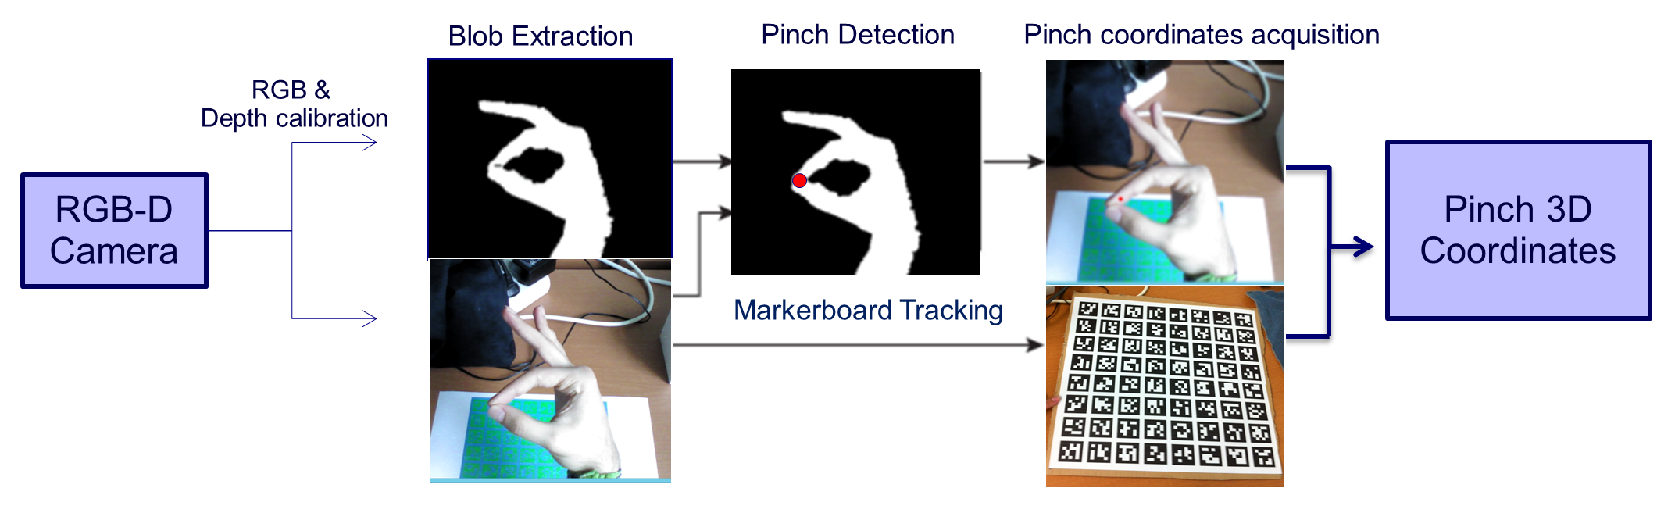
\includegraphics[width=0.9\textwidth]{Files/Figures/procedure.pdf}
    \caption[Προσέγγιση εντοπισμού σημείου χειρονομίας "τσιμπήματος" ]{Προσέγγιση εντοπισμού σημείου χειρονομίας "τσιμπήματος"}
    \label{fig:procedure}
\end{figure}



Για να δημιουργηθεί ένα σύστημα αλληλεπίδρασης ανθρώπου - υπολογιστή, οι δράσεις που παράγονται όταν λαμβάνει χώρα μία χειρονομία πρέπει να ορίζονται από ένα σύνολο καταστάσεων του συστήματος. Στις επόμενες ενότητες, θα δούμε πώς η δημιουργία τέτοιων καταστάσεων εξυπηρετεί τη λειτουργικότητα της εφαρμογής κατά τη διάρκεια ενός παιχνιδιού σκακιού επαυξημένης πραγματικότητας.





\section{Ενσωμάτωση Μηχανής Σκακιού}

Μετά την υλοποίηση του αλγορίθμου ανίχνευσης της χειρονομίας του "τσιμπήματος" και την αντιμετώπιση του προβλήματος απόκρυψης αντικειμένων, κρίθηκε απαραίτητο, ο χρήστης να μπορεί να παίξει ένα παιχνίδι σκακιού ενάντια στον υπολογιστή. Με αυτό τον τρόπο, πετυχαίνουμε μία φυσική αλληλουχία γεγονότων στο παιχνίδι του σκακιού και προσμοιώνουμε ολοκληρωμένα ένα πραγματικό παιχνίδι σκακιού απέναντι σε έναν αντίπαλο, κάτι που θα μας βοηθήσει στη συνέχεια με την αξιολόγηση του συστήματος. 


Για να μπορέσει ο χρήστης να παίξει σκάκι ενάντια στον υπολογιστή, κανονικά θα έπρεπε να υλοποιηθούν αλγόριθμοι τεχνητής νοημοσύνης που θα επέτρεπαν στο πρόγραμμα μας να καθορίσει την επόμενη κίνηση του υπολογιστή με βάση τις προηγούμενες κινήσεις που έλαβαν μέρος κατά τη διάρκεια του παιχνιδιού. Ωστόσο η υλοποίηση τέτοιων αλγορίθμων για την εφαρμογή μας δεν βρίσκεται μέσα στους σκοπούς της παρούσας διπλωματικής εργασίας και έπρεπε να αναζητηθεί ένα απλός τρόπος για την ενσωμάτωση λειτουργιών τεχνητής νοημοσύνης. 


Εκεί ακριβώς προκύπτει η λύση των μηχανών σκακιού. Μία μηχανή σκακιού δεν είναι τίποτα άλλο από ένα πρόγραμμα υπολογιστή το οποίο δέχεται σαν είσοδο την θέση ενός πιονιού στη σκακιέρα, αναλύει τις θέσεις όλων των πιονιών και υπολογίζει την καλύτερη δυνατή κίνηση με βάση τη διάταξη των πιονιών στη σκακιέρα μέσα σε ένα χρονικό περιθώριο που ορίζεται εκ των προτέρων. Η μηχανή σκακιού μπορεί να εκτιμήσει τις επόμενες κινήσεις, αλλά συνήθως δεν αλληλεπιδρά απευθείας με το χρήστη, καθώς οι περισσότερες μηχανές δεν έχουν δική τους γραφική διεπαφή για την επικοινωνία με το χρήστη. Αντίθετα οι περισσότερες είναι εφαρμογές κονσόλας που επικοινωνούν με μία γραφική διεπαφή μέσω ενός καθορισμένου πρωτοκόλλου. Αυτό επιτρέπει στο χρήστη να παίζει ενάντια σε πολλές διαφορετικές μηχανές χωρίς να χρειάζεται να εκπαιδευτεί εκ νέου σε νέες διεπαφές κάθε φορά και επιτρέπει σε διαφορετικές μηχανές να παίζουν η μία ενάντια στην άλλη. Στη συγκεκριμένη περίπτωση, η εφαρμογή μας παίζει το ρόλο της γραφικής διεπαφής ως τώρα. 


Στις μέρες μας, ο πιο πιο γνωστός τρόπος επικοινωνίας με μηχανές σκακιού πραγματοποιείται μέσω ενός πρωτοκόλλου που ονομάζεται Universal Chess Interface (UCI) Protocol. Πρόκειται για ένα πρωτόκολλο ανοιχτής επικοινωνίας που επιτρέπει σε μία μηχανή σκακιού ενός προγράμματος να επικοινωνεί με τη διεπαφή χρήστη μέσα από ένα σύνολο αυστηρά καθορισμένων εντολών. Επομένως, για να ενσωματώσουμε μία μηχανή σκακιού στην εφαρμογή μας, πρέπει να βρούμε ένα τρόπο ώστε να γίνει ανταλλαγή εντολών (συμβολοσειρές) ανάμεσα στην εφαρμογή μας και τη μηχανή σκακιού. 


Η μηχανή δέχεται εντολές μέσω standard input από μια εφαρμογή και παράγει τις απαντήσεις σε συμβολοσειρές του standard output. Δεν έχει δηλαδή γραφική διεπαφή, είσοδο μέσω ποντικιού ή εικόνες, παρά μόνο ένα απλό παράθυρο κονσόλας, που δεν είναι τίποτα περισσότερο παρά ένα εκτελέσιμο (.exe) αρχείο. 

Προκειμένου να υλοποιηθεί αυτή η επικοινωνία με το εκτελέσιμο αρχείο μιας μηχανής σκακιού αποφασίστηκε να αξιοποιηθεί η δυνατότητα που προσφέρει η βιβλιοθήκη Qt μέσω μιας κλάσης με το όνομα QProcess, η οποία επιτρέπει στο πρόγραμμά μας να εκκινήσει ένα εκτελέσιμο αρχείο, καθώς και να διαβάσει και να γράψει εντολές συμβολοσειρών από και προς αυτό. Η αλληλεπίδραση με τη μηχανή σκακιού ξεκινά με μία εντολή "uci", η οποία επικοινωνεί με τη μηχανή λέγοντας της να ταυτοποιήσει τον εαυτό της, δηλαδή να δώσει σαν έξοδο τα χαρακτηριστικά της όπως την ονομασία της, την έκδοσή της κλπ.  Έπειτα, δέχεται εντολές που μπορούν να αλλάξουν ορισμένες προεπιλεγμένες τιμές ιδιοτήτων που επηρεάζουν τα δεδομένα τα οποία θα προβάλλονται σαν έξοδος από τη μηχανή. Μετέπειτα, η μηχανή δέχεται ως είσοδο από την εφαρμογή μας την κίνηση που πραγματοποίησε ο χρήστης και εξάγει την επόμενη καλύτερη κίνηση που μπορεί να εκτελέσει ο αντίπαλος, δηλαδή ο υπολογιστής.
Η μηχανή σκακιού δέχεται σαν παράμετρο το χρόνο τον οποίο έχει για να υπολογίσει την κίνηση αυτή, ψάχνοντας για την καλύτερη δυνατή κίνηση. Ξεκινά την αναζήτηση και εκτιμά την καλύτερη κίνηση που υπάρχει πριν λήξει το χρονικό περιθώριο που ορίζεται στην αρχή της εκτέλεσης της μηχανής. 

Για την εφαρμογή μας, θεωρήσαμε ότι το χρονικό αυτό περιθώριο πρέπει να είναι ιδιαίτερα μικρό (40ms), ώστε να μην "παγώνει" η απεικόνιση των εικονικών αντικειμένων και να μπορούμε να παίρνουμε άμεσα feedback από το πρόγραμμα. Συνήθως οι μηχανές σκακιού δεν έχουν τη δυνατότητα να αντιλαμβάνονται αν μία εντολή κίνησης που δίνεται από το χρήστη είναι έγκυρη ή όχι, με βάση τον τύπο των πιονιών και την κατάσταση της σκακιέρας. Για το λόγο αυτό επιλέχθηκε να χρησιμοποιηθεί η μηχανή iCE \cite{ice}, η οποία ελέγχει αν η κίνηση που γίνεται είναι επιτρεπτή ή όχι. Αν η κίνηση δεν επιτρέπεται, τότε η μηχανή επιστρέφει ως έξοδο τη συμβολοσειρά "Invalid chess move". Αυτή η ιδιότητα επιτρέπει την υλοποίηση μιας αρχιτεκτονικής στον κώδικά μας, η οποία δε θα είναι επιρρεπής σε λανθασμένες κινήσεις όταν αυτές γίνονται κατά λάθος από το χρήστη. Επιπλέον, η μηχανή που χρησιμοποιήθηκε μπορεί να ανιχνεύσει αν το παιχνίδι ολοκληρώθηκε και ποιος είναι νικητής ώστε να μπορούμε να ενημερώσουμε το χρήστη για το αποτέλεσμα του παιχνιδιού. 

Συμπερασματικά, υλοποίησαμε τη βασική λειτουργικότητα για την αποστολή και λήψη συμβολοσειρών προς και από τη μηχανή σκακιού και με βάση αυτές τις συμβολοσειρές το πρόγραμμά μας εκτελεί συγκεκριμένες δράσεις.






\section{Χειρισμός και Απεικόνιση Εικονικών Αντικειμένων} \label{s:rendering}



Πλέον γνωρίζουμε πότε ο χρήστης πραγματοποιεί μία χειρονομία "τσιμπήματος", τη θέση του "τσιμπήματος" στον τρισδιάστατο χώρο ως προς το markerboard και πώς μπορούμε να ενσωματώσουμε μία μηχανή σκακιού για την αξιοποίηση μεθόδων τεχνητής νοημοσύνης, ώστε ο χρήστης να μπορεί να παίξει με αντίπαλο τον υπολογιστή.
Επομένως, μπορούμε να υλοποιήσουμε τη λογική του βιντεοπαιχνιδιού ενός σκακιού επαυξημένης πραγματικότητας, με στόχο τη σωστή απεικόνιση και τον χειρισμό των εικονικών αντικειμένων.


Όπως είναι ευρύτερα γνωστό, κατά τη διάρκεια ενός παιχνιδιού σκακιού πραγματοποιούνται διαδοχικές κινήσεις από τους 2 παίκτες. Ένας παίκτης μπορεί να μετακινήσει ένα πιόνι με βάση τον τύπο του και τις ιδιότητές του, που του επιτρέπουν να κινηθεί σε συγκεκριμένα τετράγωνα της σκακιέρας ή να αιχμαλωτίσει ένα αντίπαλο πιόνι και να τοποθετηθεί στο τετράγωνο εκείνο. Επιπλέον υπάρχουν ορισμένες ειδικές κινήσεις όπως το ροκέ, όπου πραγματοποιείται μετακίνηση του βασιλιά δύο τετράγωνα προς τον πύργο και μετακίνηση του πύργου στο τετράγωνο ανάμεσα στην αρχική και τελική θέση του βασιλιά. Είναι η μοναδική κίνηση στο σκάκι, που κάποιος παίκτης μπορεί να μετακινήσει στη σειρά του, ταυτόχρονα δύο πιόνια.

Πιο συγκεκριμένα, όταν ένας χρήστης επιχειρήσει μία χειρονομία "τσιμπήματος" με στόχο να μετακινήσει ένα πιόνι, πρέπει το πιόνι να απεικονίζεται ως προς το σημείο όπου πραγματοποιήθηκε η χειρονομία ώστε να κινείται όπως κινείται και το χέρι του χρήστη.
Αν ο χρήστης αποφασίσει να ολοκληρώσει μία κίνηση, πρέπει να μετακινήσει το πιόνι πάνω από ένα άλλο τετράγωνο της σκακιέρας και να πραγματοποιήσει μία κίνηση αντίθετη της χειρονομίας "τσιμπήματος" που υποδεικνύει απελευθέρωση του αντικειμένου (pinch-out). Η κίνηση αυτή πραγματοποιείται όταν ο δείκτης και ο αντίχειρας παύουν να αγγίζουν ο ένας τον άλλον.  
Μόλις η κίνηση αυτή πραγματοποιηθεί και αν είναι έγκυρη, πρέπει το σύστημα να απευθυνθεί στη μηχανή σκακιού και να μάθει την καλύτερη κίνηση που προτείνεται για τον αντίπαλο μέσω των αλγορίθμων τεχνητής νοημοσύνης. 
Μόλις η μηχανή απαντήσει, έχουμε ουσιαστικά μία κίνηση που πρέπει να πραγματοποιηθεί από τα αντίπαλα πιόνια και επομένως πρέπει να ανανεωθεί η σκακιέρα και η θέση των πιονιών πάνω σε αυτή. 

Αυτή η αλληλουχία γεγονότων που αναφέρθηκε είναι αρκετά πολύπλοκο να υλοποιηθεί απευθείας, επομένως αποφασίστηκε να εκτελούνται διαφορετικές εντολές με βάση την κατάσταση του παιχνιδιού σε κάθε χρονική στιγμή και το αν έχει ανιχνευθεί μία χειρονομία "τσιμπήματος".

Συγκεκριμένα, όταν ενεργοποιείται μία "σημαία" που υποδεικνύει ότι ανιχνεύθηκε ένα "τσίμπημα" σε κάθε frame, πρέπει να αλλάζει η κατάσταση του συστήματος λαμβάνοντας υπόψη ορισμένες παραμέτρους.

Υπάρχουν 5 βασικές καταστάσεις στην υλοποίηση που προτείνεται με τις ονομασίες Free, Pinch-In, Pinch-Continuous, Pinch-Out και enemy-Move. 

Όπως φαίνεται και από το διάγραμμα~\ref{fig:states}, η κατάσταση του συστήματος αλλάζει με βάση την προηγούμενη κατάσταση του προγράμματος και συγκεκριμένες παραμέτρους. Αφού έγινε ανάλυση της κίνησης ενός παίκτη προσεκτικά, υλοποιήθηκαν οι καταστάσεις που περιγράφονται αναλυτικά παρακάτω:

\begin{enumerate}
\item \textbf{FREE}: Ο χρήστης δεν πραγματοποιεί καμία χειρονομία ή το σύστημα δεν μπορεί να εντοπίσει καμία χειρονομία τσιμπήματος στο συγκεκριμένο frame.

\item \textbf{PINCH-IN}: Ανιχνεύθηκε μία χειρονομία τσιμπήματος και επομένως, αν η προηγούμενη κατάσταση του συστήματος είναι η FREE, η παρούσα κατάσταση μετατρέπεται σε PINCH-IN.


\item \textbf{PINCH-CONTINUOUS}: Ανιχνεύθηκε μία χειρονομία τσιμπήματος και αν η προηγούμενη κατάσταση του συστήματος είναι η PINCH-IN, η παρούσα κατάσταση μετατρέπεται σε PINCH-CONTINUOUS. Αυτό σημαίνει ότι ο χρήστης μπορεί να θέλει να μετακινήσει ένα εικονικό πιόνι. 

\item \textbf{PINCH-OUT}: Δεν υπάρχει ανίχνευση χειρονομίας τσιμπήματος για έναν συγκεκριμένο αριθμό διαδοχικών frames. Η προηγούμενη κατάσταση είναι είτε Pinch-In ή Pinch-Continuous, επομένως μπορεί να έχουμε μία ολοκληρωμένη κίνηση από το χρήστη. 


\item \textbf{ENEMY-MOVE}: Το σύστημα εισέρχεται σε αυτή την κατάσταση μετά από κάθε κατάσταση PINCH-OUT και αν η κίνηση είναι που πραγματοποιήθηκε θεωρείται έγκυρη. Επίσης το σύστημα παραμένει σε αυτή την κατάσταση όσο διαρκεί το animation της κίνησης του πιονιού του αντιπάλου, δηλαδή του υπολογιστή. 
\end{enumerate}




\begin{figure}[H]
    \centering
    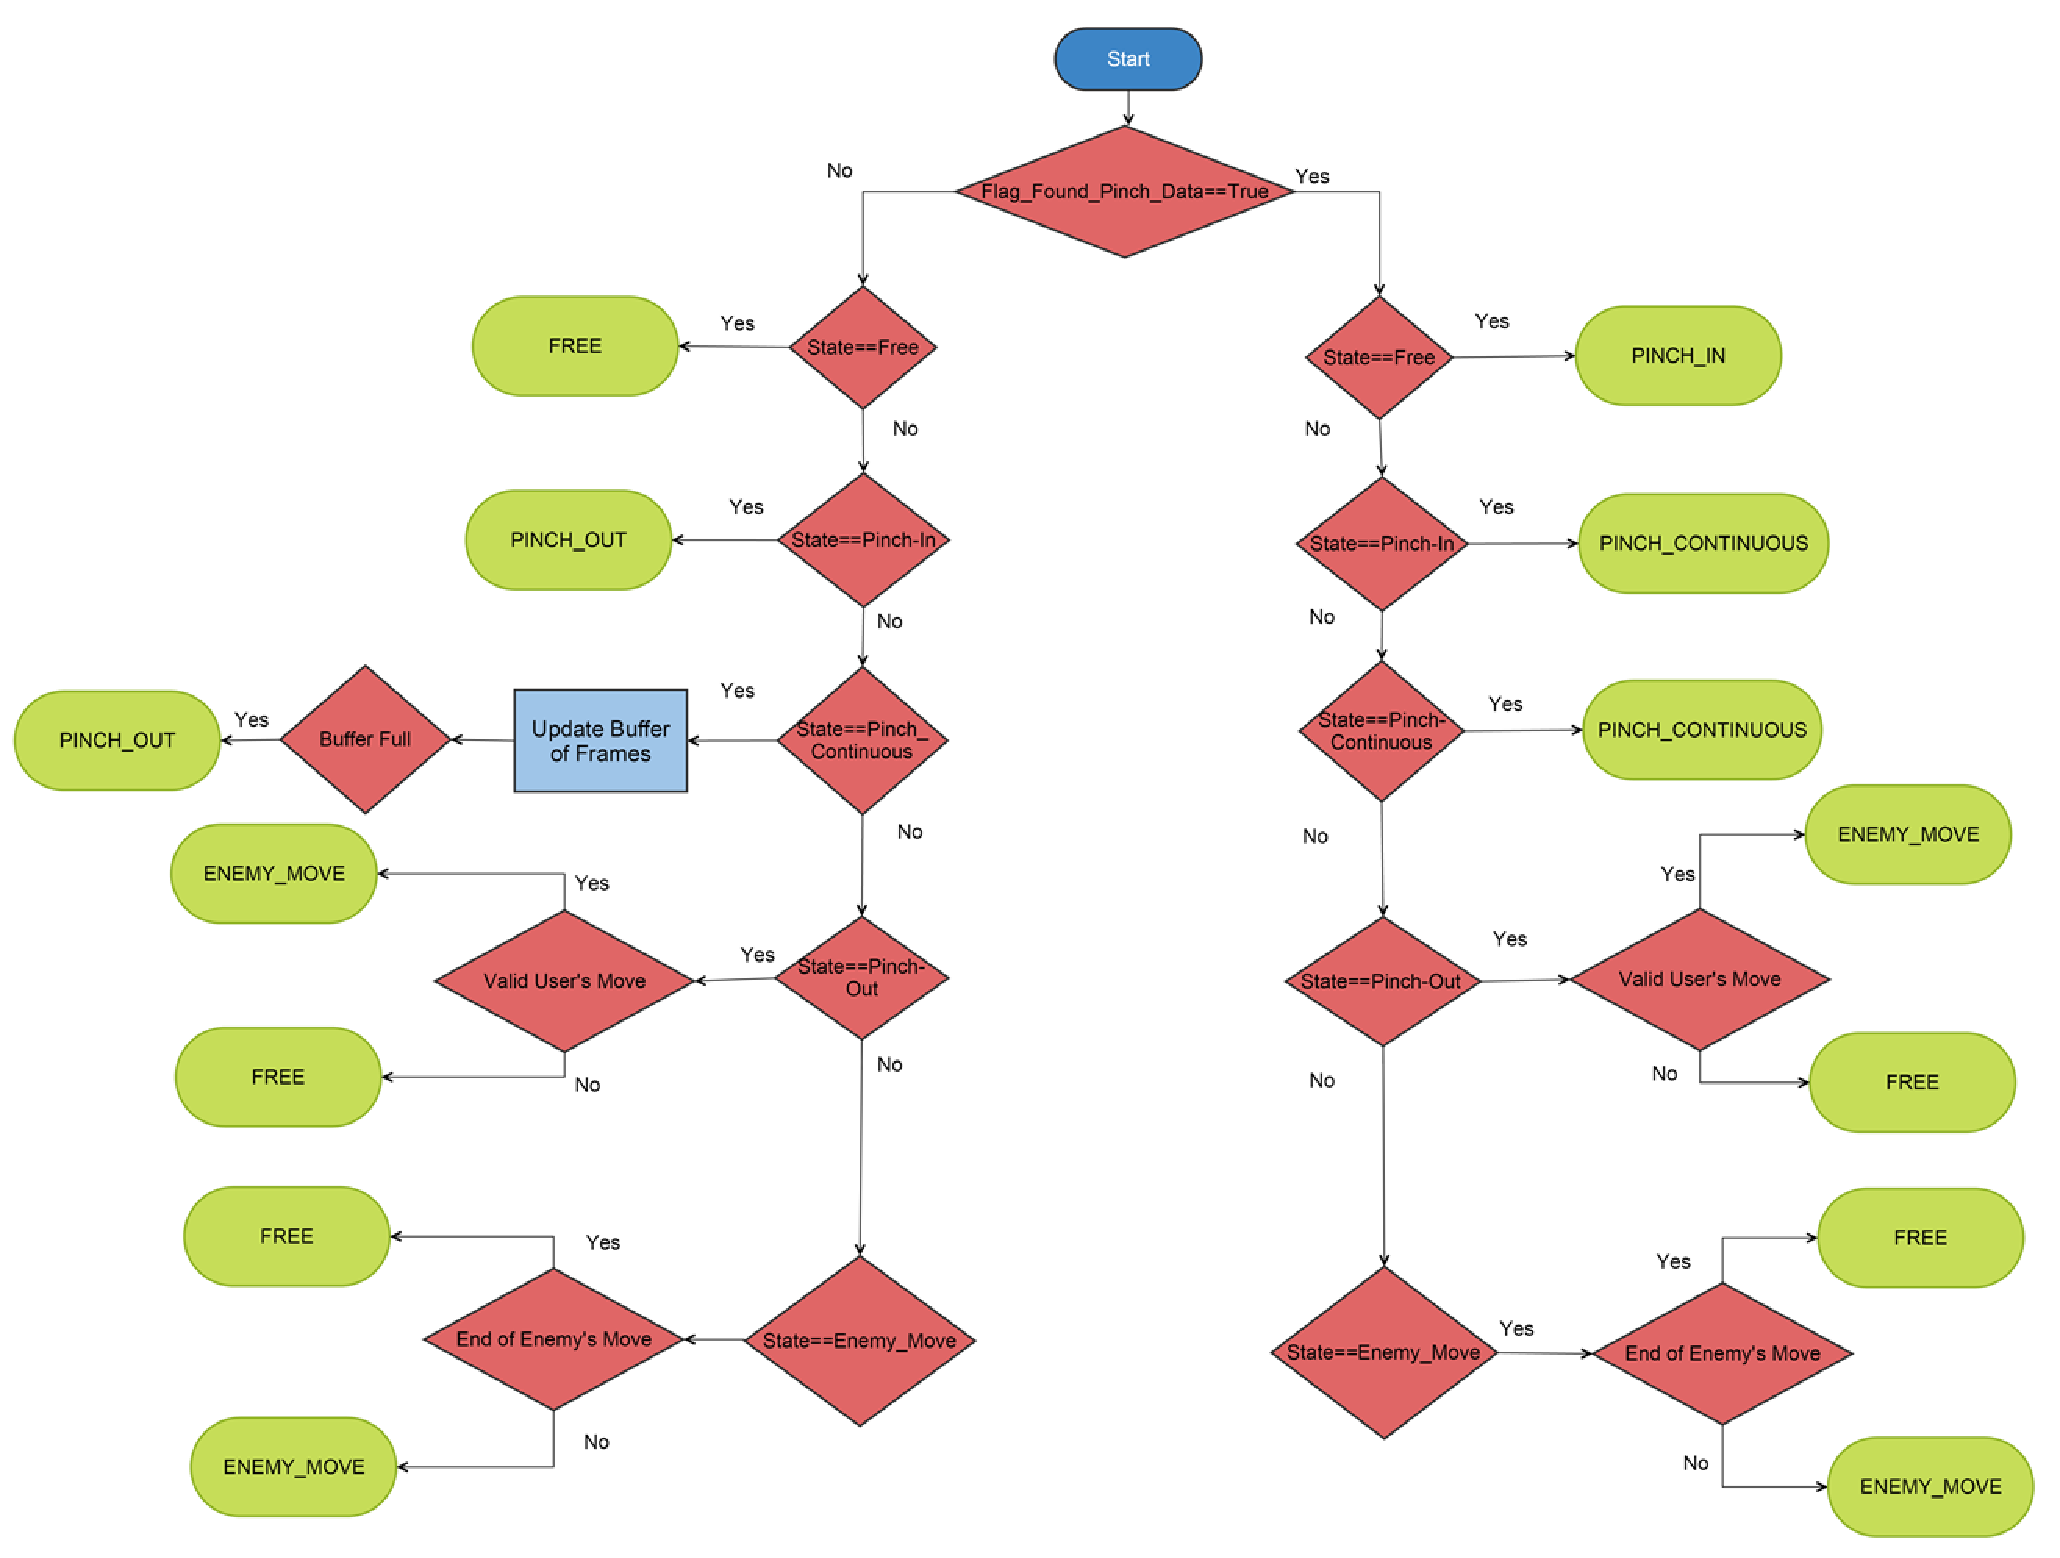
\includegraphics[width=0.95\textwidth]{Files/Figures/change_of_states.pdf}
    \caption[Διάγραμμα του αλγορίθμου αλλαγής καταστάσεων της εφαρμογής]{Διάγραμμα του αλγορίθμου αλλαγής καταστάσεων της εφαρμογής}
    \label{fig:states}
\end{figure}






Αφού το σύστημα εισέλθει σε μία συγκεκριμένη κατάσταση, μπορούμε στη συνέχεια να εκτελέσουμε εντολές με τις οποίες τα εικονικά πιόνια θα απεικονιστούν ή όχι. Το κομμάτι αυτό είναι ιδιαίτερα σημαντικό, καθώς για παράδειγμα, όταν ένα πιόνι αιχμαλωτίζει ένα άλλο, τότε αυτό πρέπει να σταματήσει να απεικονίζεται στη σκακιέρα.


Συγκεκριμένα, αν η τρέχουσα κατάσταση του συστήματος είναι η Free, τότε χρειάζεται να απεικονίσουμε κάθε εικονικό πιόνι που υπάρχει στην εσωτερική αναπαράσταση της σκακιέρας, δηλαδή σε μία δομή δεδομένων που αποτελείται από ένα πίνακα με δείκτες προς μεταβλητές που προσομοιώνουν τα πιόνια και τις ιδιότητές τους. Με βάση τον τύπο κάθε πιονιού, μπορούμε να απεικονίσουμε το σωστό 3D μοντέλο (π.χ βασίλισσα, αξιωματικός κ.λπ) πάνω από το κατάλληλο τετράγωνο της σκακιέρας. 


\begin{figure}[H]
    \centering
    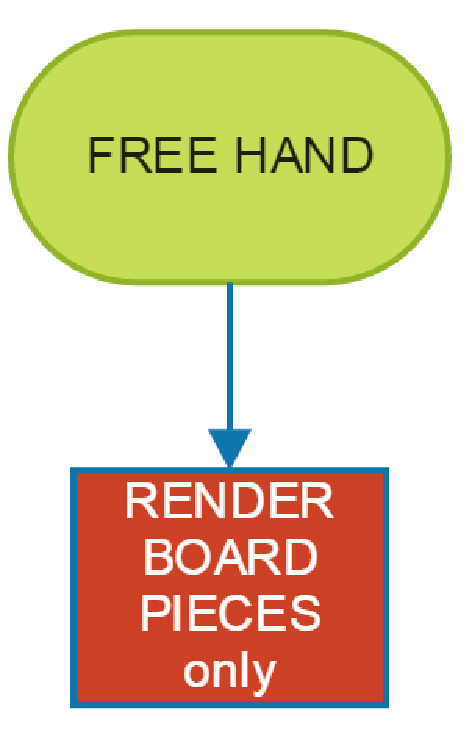
\includegraphics[scale=0.35, angle=0]{Files/Figures/free_hand.pdf}
    \caption[Διάγραμμα ροής κατάστασης Free]{[Διάγραμμα ροής κατάστασης Free}
    \label{fig:free}
\end{figure}



Όταν η τρέχουσα κατάσταση είναι η Pinch-In, τότε ο χρήστης μπορεί να θέλει να επιλέξει ένα πιόνι. Ωστόσο πρέπει με ακρίβεια να εντοπίσουμε ποιο πιόνι είναι αυτό το οποίο προσπαθεί να επιλέξει ο χρήστης από όλα αυτά που υπάρχουν στη σκακιέρα σε κάθε χρονική στιγμή. 

Για να συμβεί αυτό, ακολουθείται μία διαδικασία κατά την οποία, με βάση την θέση στην οποία συνέβη το "τσίμπημα" στον τρισδιάστατο χώρο, υπολογίζουμε όλες τις ευκλείδιες αποστάσεις από αυτή και το κέντρο όλων των τετραγώνων της σκακιέρας, τα οποία έχουν ένα πιόνι επάνω τους και αυτό το πιόνι ανήκει στο χρήστη και όχι στον υπολογιστή. Από το σύνολο των τιμών αυτών των αποστάσεων, βρίσκουμε το τετράγωνο εκείνο το οποίο απέχει λιγότερο από το σημείο "τσιμπήματος", καθώς και την τιμή της απόστασης σε μέτρα. 



Ωστόσο, για να αποτραπεί η επιλογή ενός πιονιού, όταν η χειρονομία του χρήστη γίνεται αρκετά μακριά από τα εικονικά πιόνια ή ακόμα και εκτός της σκακιέρας, χρειάζεται να ικανοποιείται μία συνθήκη, ώστε η απόσταση αυτή η οποία ορίστηκε ως μικρότερη, να είναι και μικρότερη από μία τιμή, η οποία εκτιμήθηκε μετά από δοκιμές.


Αν η επιλογή του πιονιού θεωρηθεί από τον αλγόριθμο αυτό ως έγκυρη, τότε κατά τη διαδικασία του σχεδιασμού των πιονιών μέσω της OpenGL, θα απεικονίσουμε όλα τα πιόνια της σκακιέρας, εκτός από αυτό που επιλέχθηκε. Αυτό το οποίο επιλέχθηκε, αντίθετα, θα απεικονιστεί στην επαυξημένη σκηνή, αλλά όχι στατικό πάνω από το τετράγωνο, αλλά στη θέση όπου έγινε η χειρονομία "τσιμπήματος" του χρήστη. Σε αντίθετη περίπτωση, δεν έχουμε έγκυρη επιλογή πιονιού, επειδή ο χρήστης προσπάθησε να επιλέξει ένα πιόνι πιο μακριά από ότι έπρεπε στη σκακιέρα και επομένως απεικονίζονται στην επαυξημένη σκηνή όλα τα πιόνια τα οποία βρίσκονται στη σκακιέρα την τρέχουσα χρονική στιγμή (όσα δεν έχουν αιχμαλωτιστεί κλπ).




\begin{figure}[H]
    \centering
    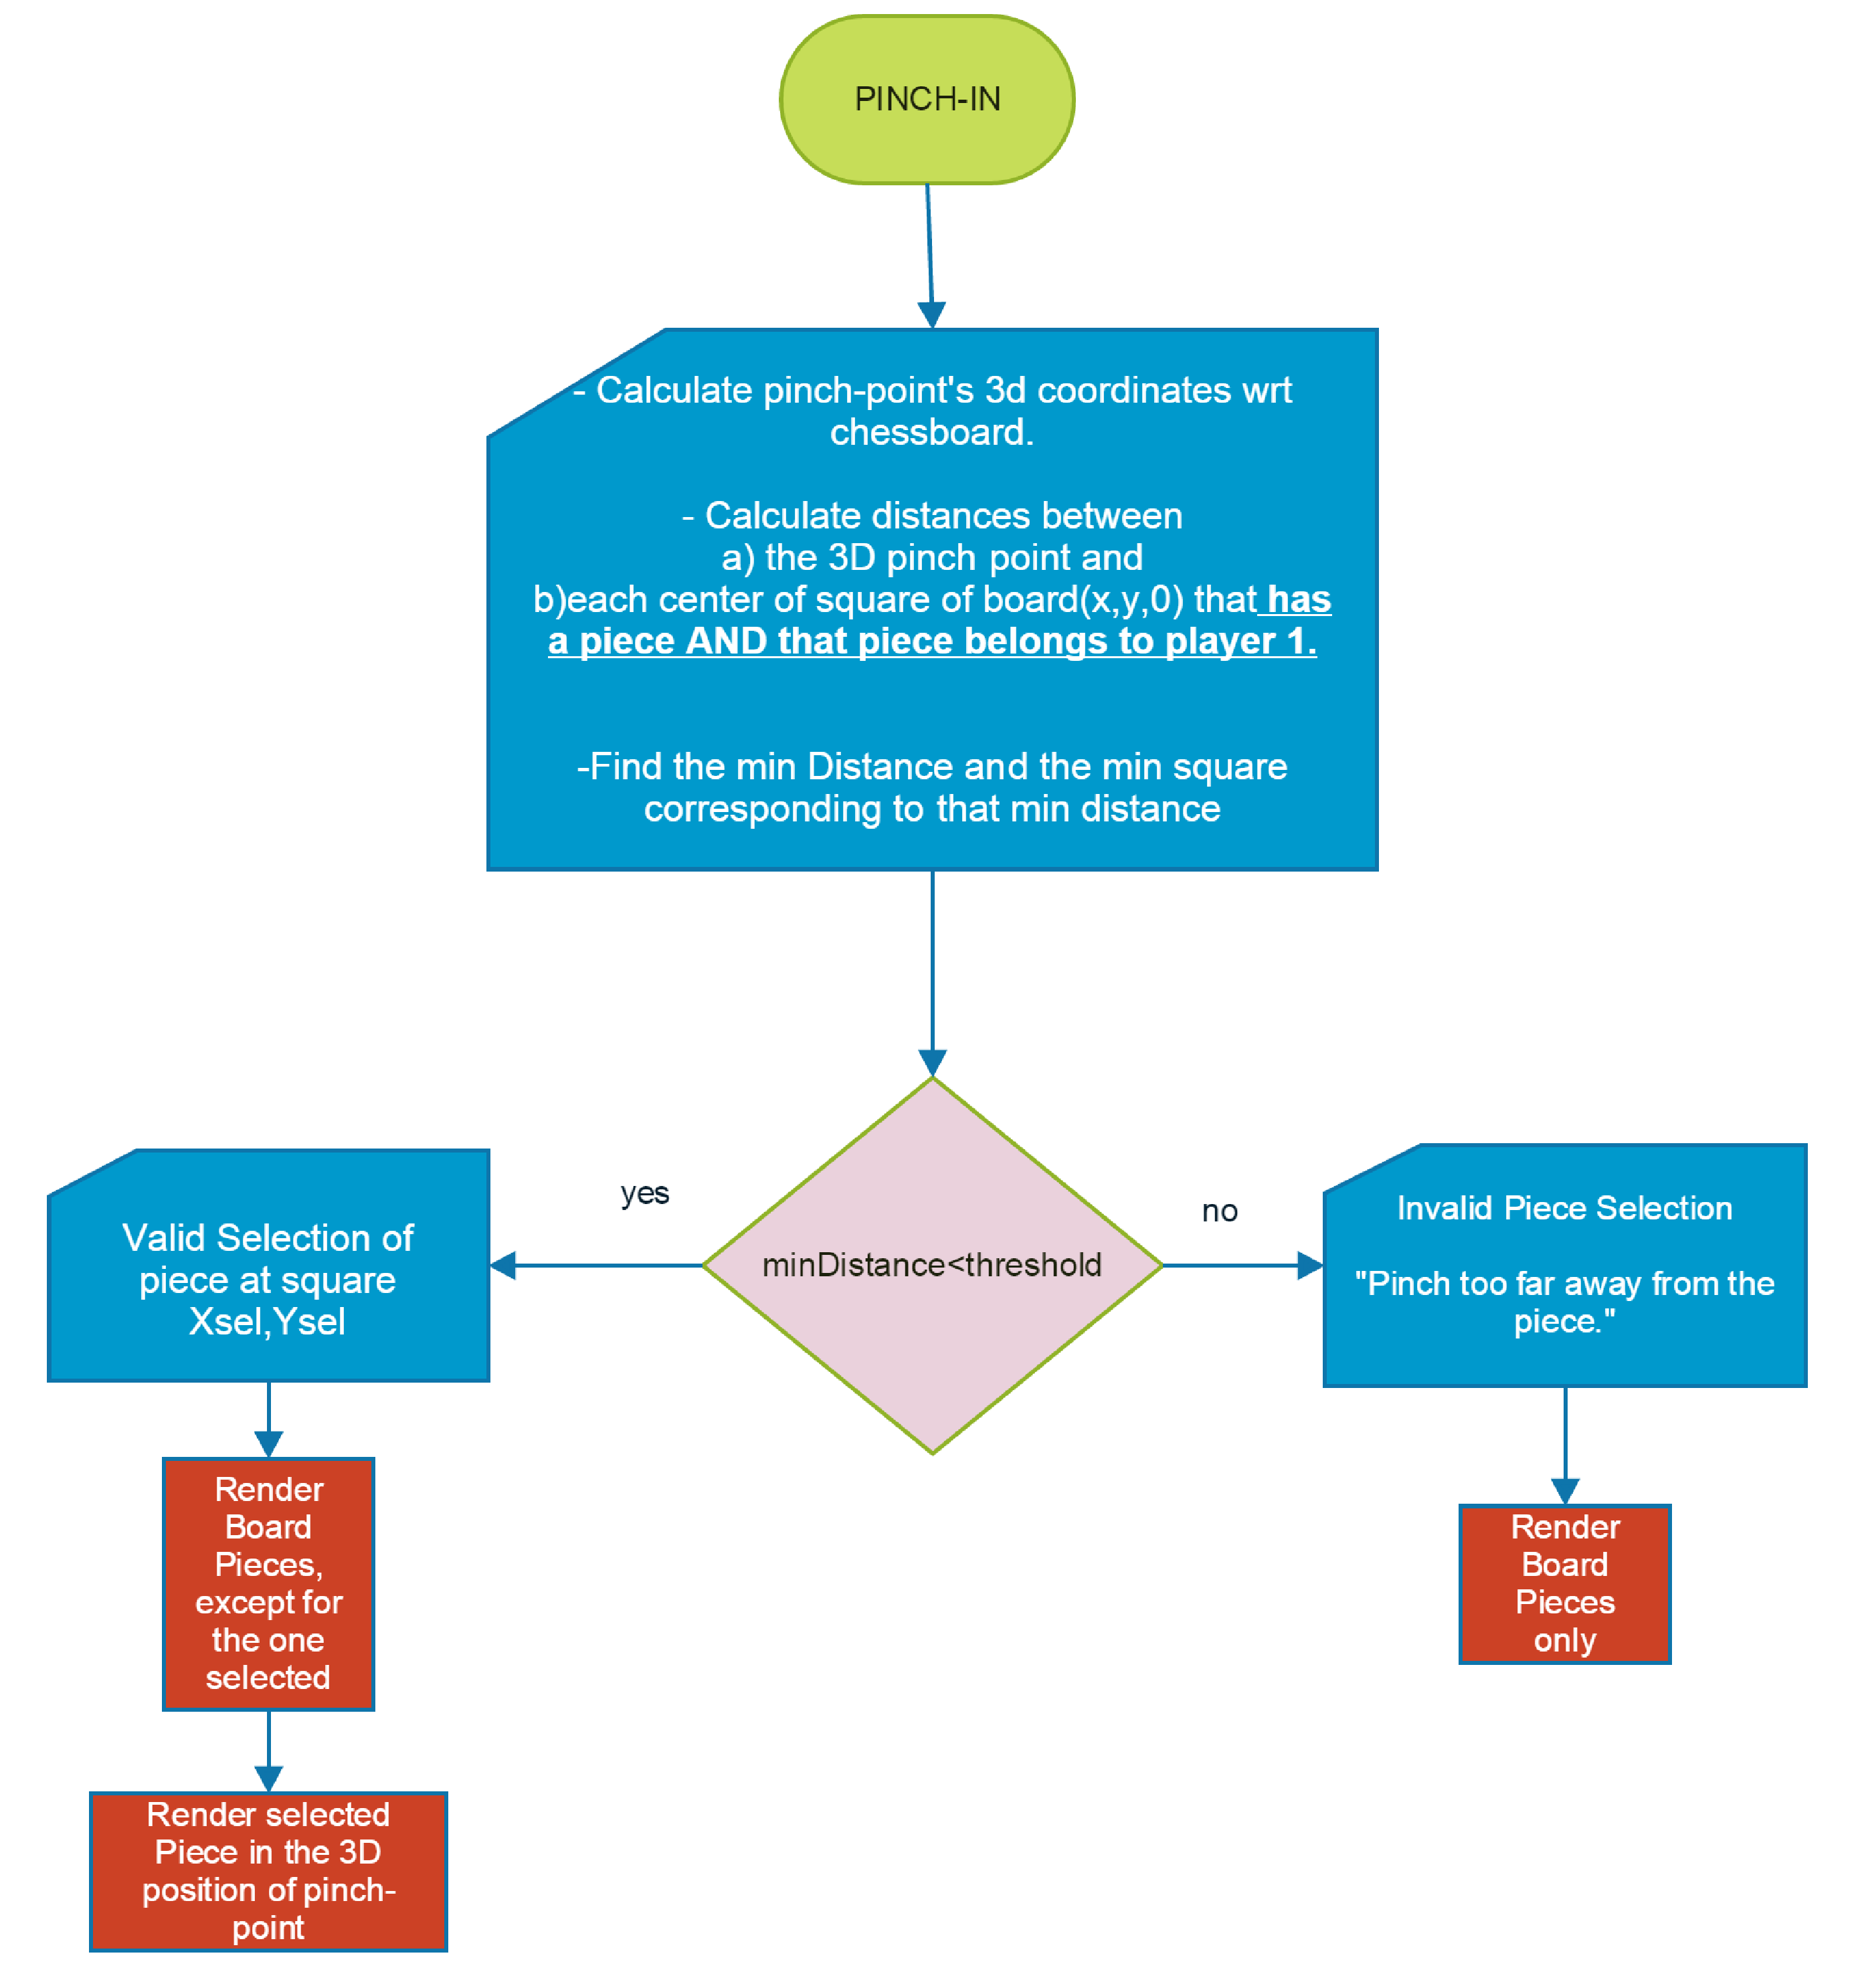
\includegraphics[width=0.86\textwidth]{Files/Figures/pinch_in.pdf}
    \caption[Διάγραμμα ροής κατάστασης Pinch-In]{Διάγραμμα ροής κατάστασης Pinch-In}
    \label{fig:pinch-in}
\end{figure}


Όταν η κατάσταση του συστήματος είναι η Pinch-Continuous, τότε αν στην προηγούμενη κατάσταση είχαμε έγκυρη επιλογή ενός πιονιού, θα απεικονιστούν όλα τα πιόνια της σκακιέρας, εκτός από αυτό που επιλέχθηκε, το οποίο θα απεικονιστεί ως προς το σημείο "τσιμπήματος". 

\begin{figure}[H]
    \centering
    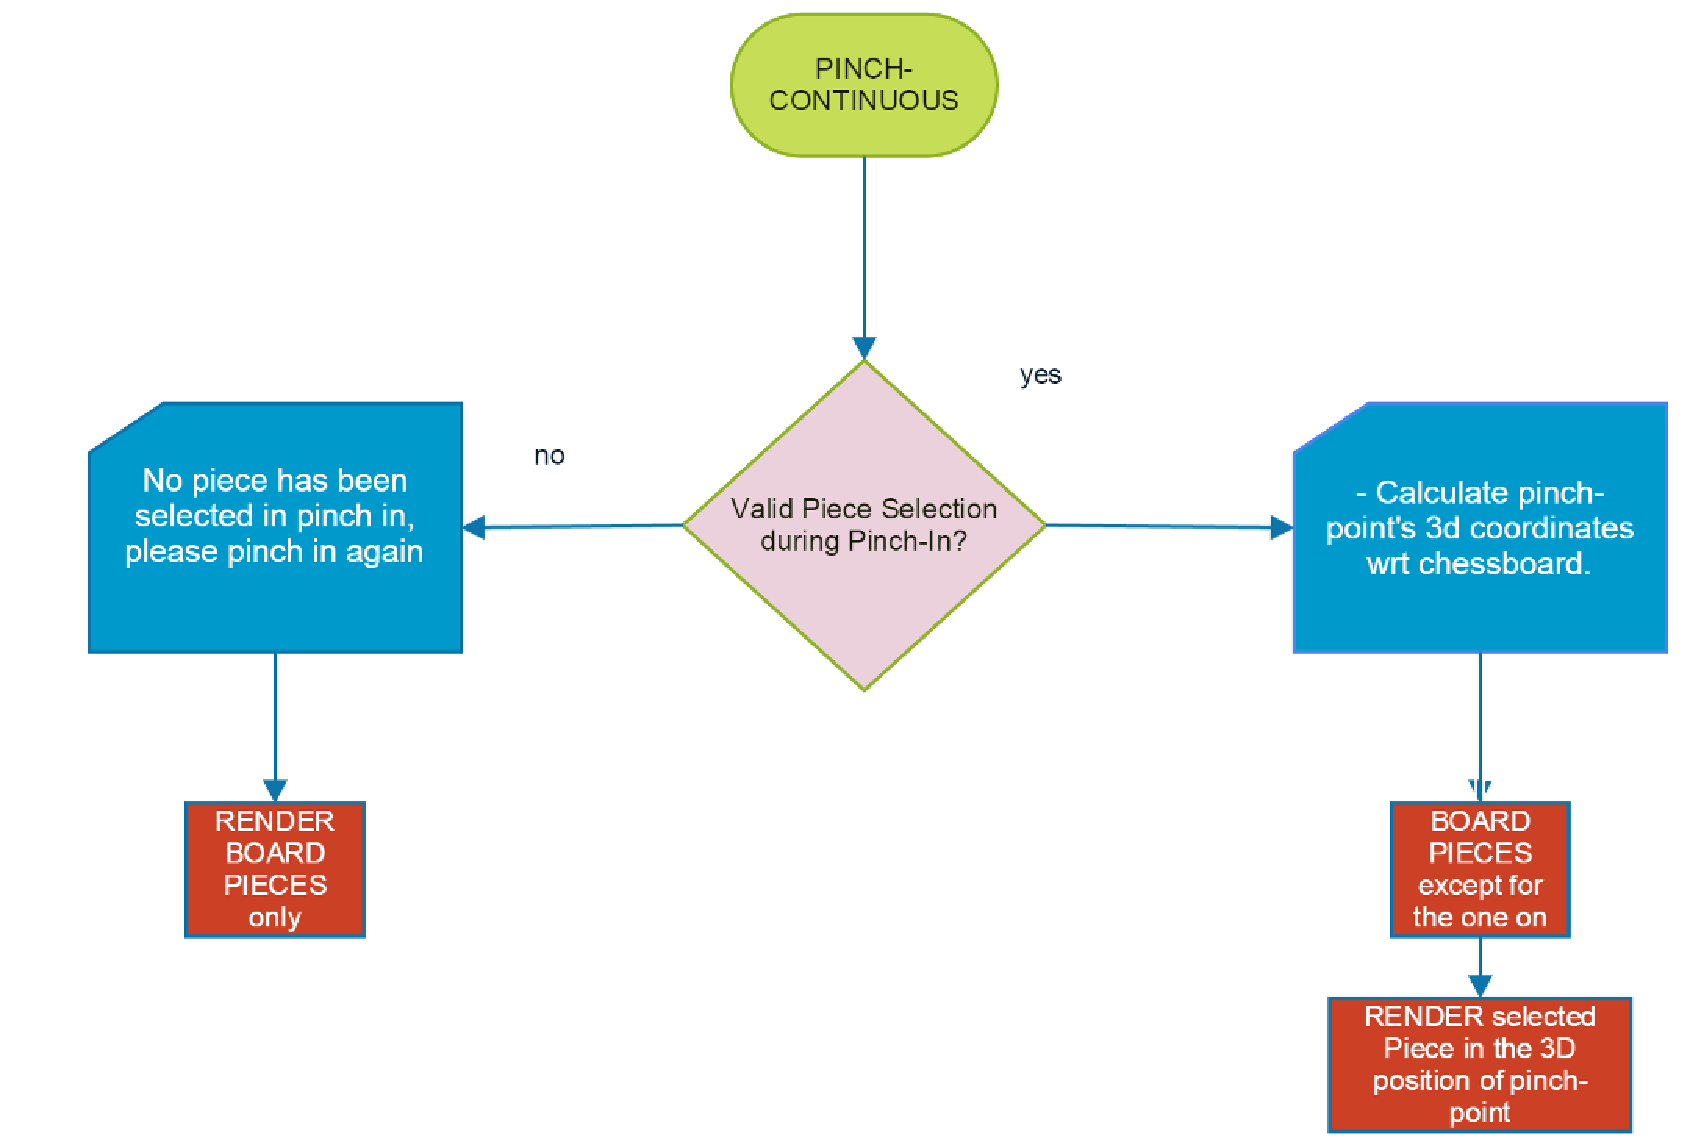
\includegraphics[width=0.95\textwidth]{Files/Figures/pinch_continuous_state.pdf}
    \caption[Διάγραμμα ροής κατάστασης Pinch-Continuous]{Διάγραμμα ροής κατάστασης Pinch-Continuous}
    \label{fig:pinch-continuous}
\end{figure}



Αφού διαπιστωθεί αν επιλέχθηκε έγκυρα ένα πιόνι στις προηγούμενες καταστάσεις, στην κατάσταση Pinch-Out πρέπει να βρεθεί το σημείο εκείνο στη σκακιέρα όπου ο χρήστης επέλεξε να αφήσει το πιόνι το οποίο μετακινεί. Το πιόνι αυτό, έπειτα, πρέπει να ανατεθεί στο νέο τετράγωνο της σκακιέρας και να ανανεωθεί η δομή της σκακιέρας και η διάταξη των πιονιών.

Για να πραγματοποιηθεί αυτή η διαδικασία, πρέπει αρχικά να υπολογιστούν οι αποστάσεις ανάμεσα στην προβολή του τελευταίου σημείου "τσιμπήματος" που ανιχνεύθηκε πριν απελευθερώσει ο χρήστης τον αντίχειρα και το δείκτη του και το κέντρο κάθε τετραγώνου της σκακιέρας, όπου υπάρχει αντίπαλο πιόνι ή ελεύθερο τετράγωνο. Στη συνέχεια, παίρνουμε τις συντεταγμένες του τετραγώνου που βρίσκεται πιο κοντά στην προβολή του σημείου "τσιμπήματος". Το συγκεκριμένο τετράγωνο θα θεωρηθεί ως το τετράγωνο τελικής θέσης του πιονιού. 


Μόλις επιλεγεί το συγκεκριμένο τετράγωνο, ουσιαστικά έχουμε μία ολοκληρωμένη κίνηση που προσπαθεί να πραγματοποιήσει ο χρήστης. Ωστόσο, αυτή η κίνηση μπορεί να μην είναι έγκυρη με βάση τους κανόνες που ισχύουν στο σκάκι. Για παράδειγμα ο χρήστης μπορεί να προσπαθήσει να μετακινήσει τον βασιλιά 3 ή περισσότερα τετράγωνα μακριά από την αρχική του θέση. Για να αντιμετωπιστεί το συγκεκριμένο πρόβλημα, πρέπει να γίνεται έλεγχος της εγκυρότητας κάθε κίνησης μέσω της μηχανής σκακιού που χρησιμοποιείται (iCE Engine). 


Πιο συγκεκριμένα, πρέπει αρχικά να μετασχηματίσουμε την κίνηση που πραγματοποίησε ο χρήστης στη σκακιέρα και η οποία αναπαρίσταται από 4 αριθμούς που δείχνουν τις αρχικές και τις τελικές συντεταγμένες του τετραγώνου στο 8 x 8 πλέγμα της σκακιέρας σε μία συμβολοσειρά που είναι συμβατή με το πρωτόκολλο UCI (π.χ ο αριθμός 0102 γίνεται A2A3). Με αυτόν τον τρόπο παίρνουμε μία απάντηση από τη μηχανή σχετικά με το αν η κίνηση του χρήστη είναι έγκυρη ή όχι. 


Αν η κίνηση δεν είναι έγκυρη, τότε δε χρειάζεται να ανανεωθεί η εσωτερική αναπαράσταση της διάταξης των πιονιών στη σκακιέρα και το πιόνι που έγινε προσπάθεια να μετακινηθεί, επιστρέφει πίσω στην αρχική του θέση. Διαφορετικά, έχουμε μία έγκυρη κίνηση, πηγαίνουμε στην επόμενη κατάσταση που είναι η Enemy-Move και ανανεώνεται η θέση του πιονιού που κινείται στην εσωτερική αναπαράσταση της διάταξης των πιονιών. Τέλος απεικονίζονται στην οθόνη, όλα τα πιόνια που ανήκουν στη σκακιέρα.


\begin{figure}[H]
    \centering
    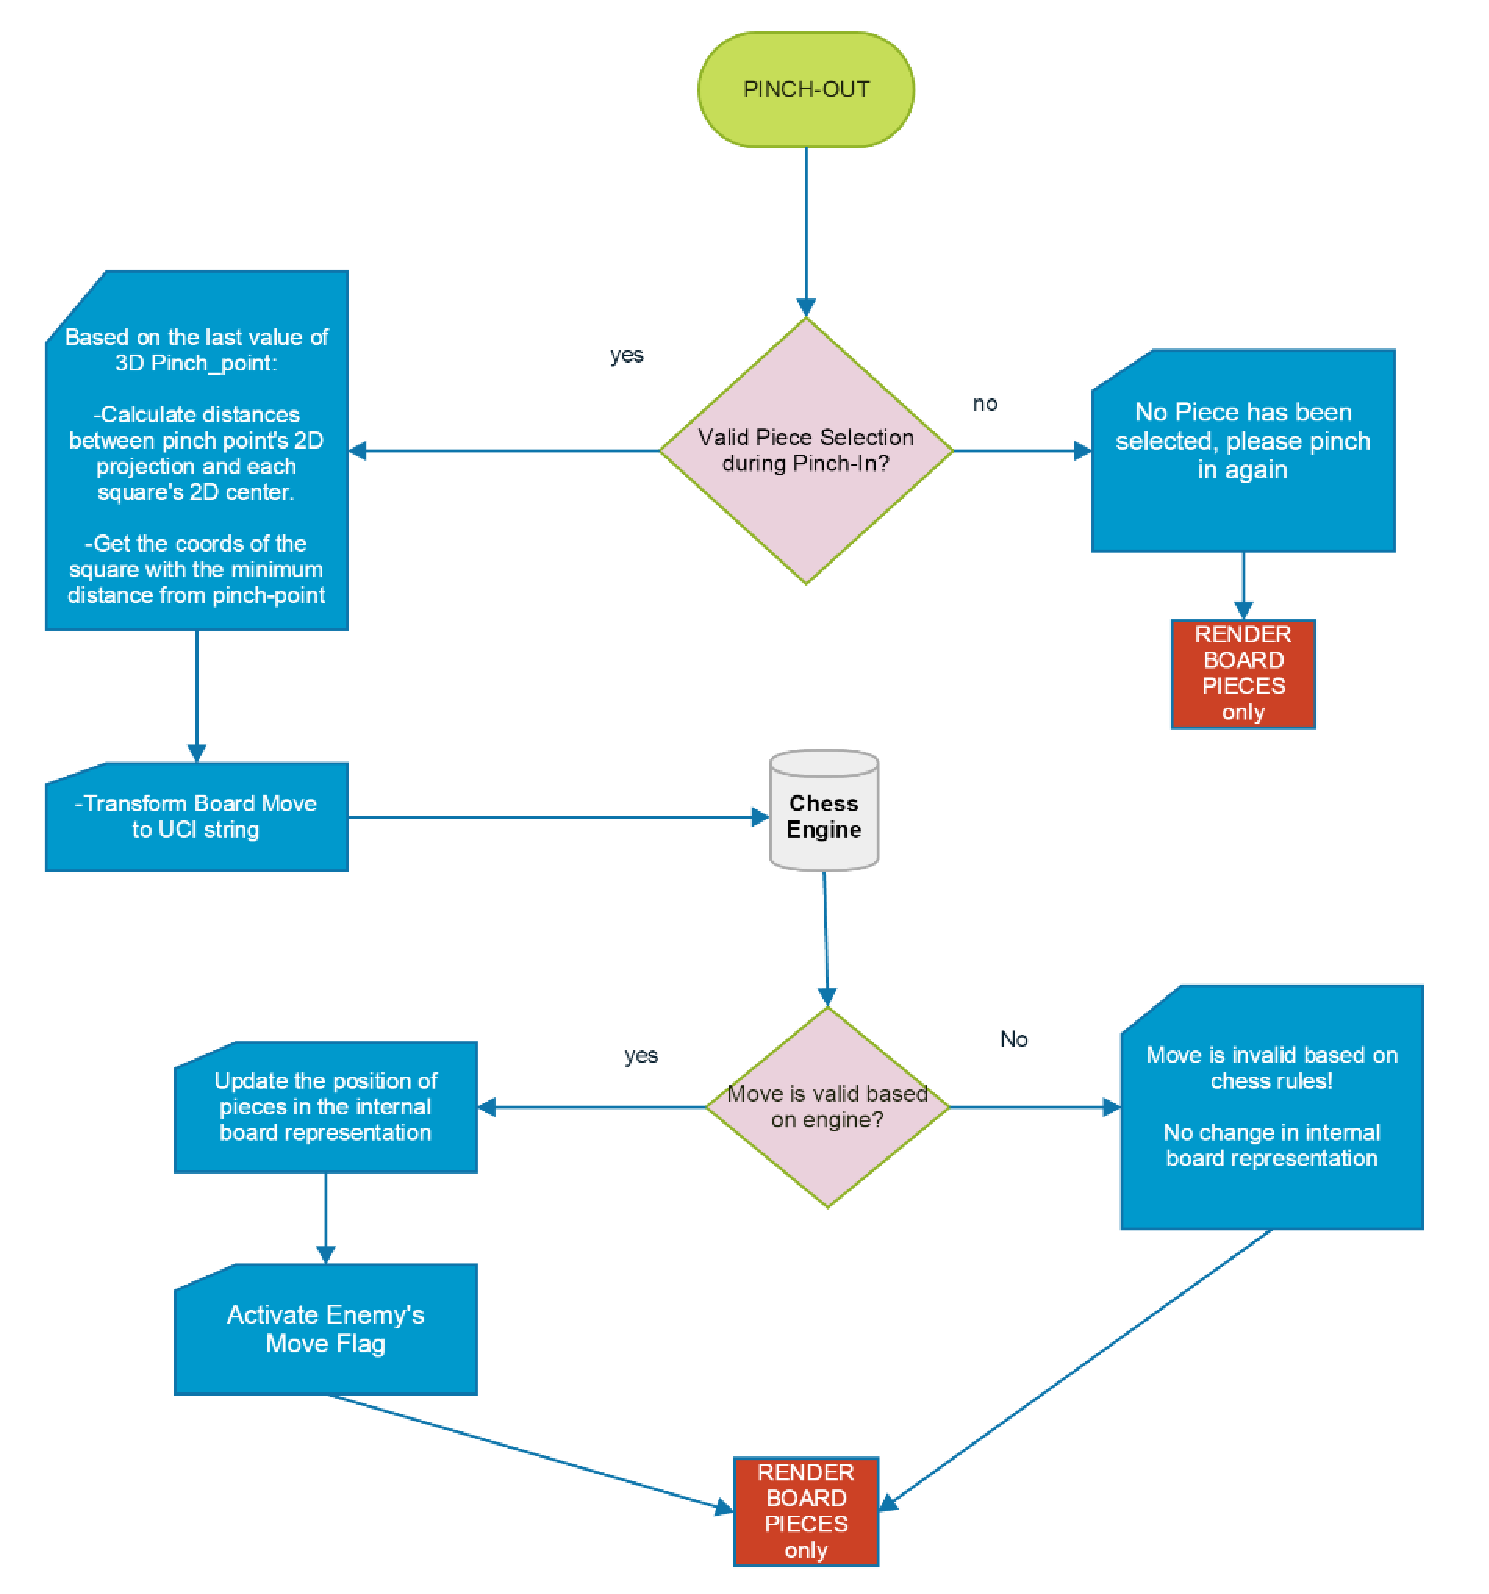
\includegraphics[width=0.85\textwidth]{Files/Figures/pinch_out.pdf}
    \caption[Διάγραμμα ροής κατάστασης Pinch-Out]{Διάγραμμα ροής κατάστασης Pinch-Out}
    \label{fig:pinch_out}
\end{figure}



Η τελευταία κατάσταση, για να ολοκληρωθεί ένα γύρος του παιχνιδιού, είναι η Enemy-Move, όπου χρειάζεται η εκτίμηση μιας κίνησης από τη μηχανή σκακιού για τα πιόνια του αντιπάλου. Η κίνηση, όπως αυτή παράγεται από τη μηχανή, εμφανίζεται σε μορφή συμβατή με το πρωτόκολλο UCI. Επομένως χρειάζεται ένας απλός μετασχηματισμός, από μία συμβολοσειρά σε μία σειρά αριθμών που θα δοθούν ως είσοδος στην εσωτερική δομή της διάταξης για να πραγματοποιηθεί μία κίνηση.
Έπειτα, ξεκινά to animation της κίνησης του πιονιού του αντιπάλου, που βασίζεται στην αρχή της παρεμβολής ανάμεσα στην αρχικό και το τελικό τετράγωνο της κίνησης. Τελικά, απεικονίζονται όλα τα πιόνια της ανανεωμένης διάταξης πιονιών.


\begin{figure}[H]
    \centering
    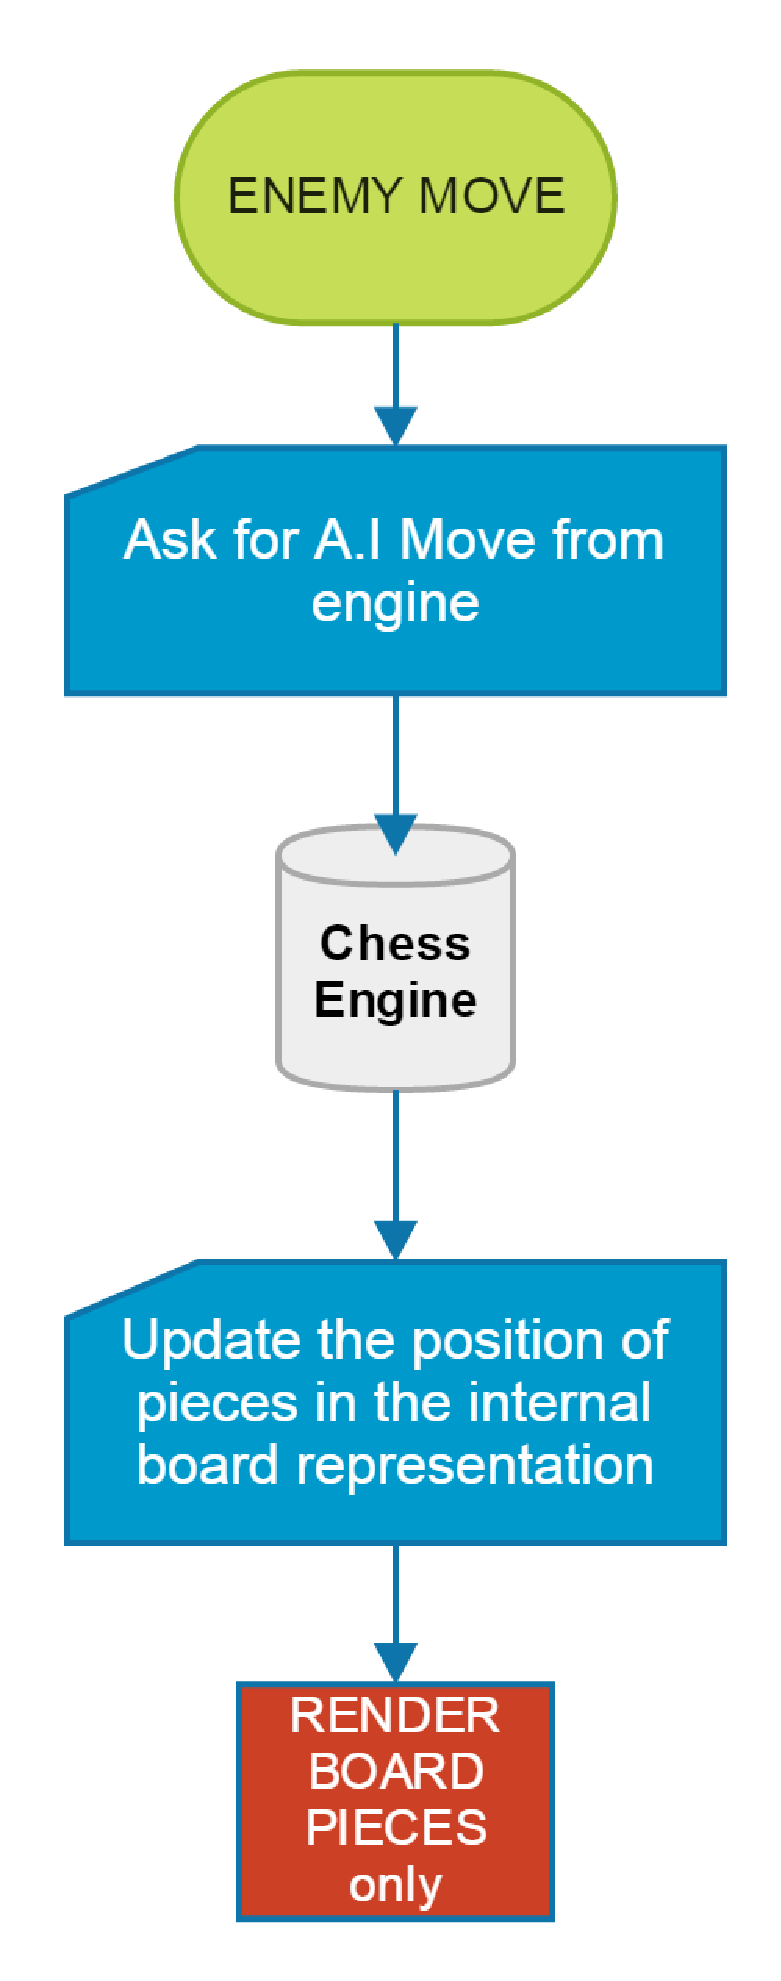
\includegraphics[scale=0.3]{Files/Figures/enemy_move.pdf}
    \caption[Διάγραμμα ροής κατάστασης Enemy-Move]{Διάγραμμα ροής κατάστασης Enemy-Move}
    \label{fig:enemy_move}
\end{figure}


\section{Αντιμετώπιση Απόκρυψης Αντικειμένων} \label{s:occlusion}




%-----
Για να μπορέσει ένας χρήστης να εκτελέσει επιτυχώς ορισμένες διεργασίες σε περιβάλλοντα επαυξημένης πραγματικότητας, χρειάζεται να παρέχεται από το σύστημα ένα συγκεκριμένο επίπεδο "εμβύθισης" του χρήστη. Πρέπει δηλαδή ο χρήστης να πιστέψει, όσο γίνεται, ότι τα εικονικά αντικείμενα είναι πραγματικά. 


Στις περισσότερες προσεγγίσεις, οι αποκρύψεις των εικονικών αντικειμένων δεν λαμβάνονται υπόψη και επομένως τα εικονικά αντικείμενα απεικονίζονται πάντα πάνω από το frame του βίντεο, συνεπώς πάνω από τα πραγματικά αντικείμενα της σκηνής. 
Ωστόσο, για να δημιουργηθούν καθηλωτικές και ρεαλιστικές εφαρμογές, η απόκρυψη ανάμεσα στα εικονικά και τα πραγματικά αντικείμενα πρέπει να πραγματοποιηθεί σωστά, ώστε οι χρήστες να μπορούν να κοιτάξουν σε μία σκηνή, όπου το εικονικό περιεχόμενο θα είναι εναρμονισμένο με το φυσικό περιβάλλον. Μία τέτοια προσέγγιση μας επιτρέπει να πετύχουμε υψηλό επίπεδο "εμβύθισης" αφού τα εικονικά αντικείμενα μπορούν να εναρμονιστούν με τα χέρια του χρήστη, ώστε να εμφανίζεται σωστά το ένα πάνω από το άλλο ή το αντίθετο. 

Κάτι τέτοιο συνήθως δε συμβαίνει στις περισσότερες εφαρμογές επαυξημένης πραγματικότητας. Στην OpenGL, όταν ένα αντικείμενο απεικονίζεται στην οθόνη, το βάθος ενός pixel που παράγεται (z coordinate) αποθηκεύεται σε ένα buffer που ονομάζεται z-buffer ή buffer βάθους (depth buffer). Αυτός ο buffer ορίζεται συνήθως ως ένα δισδιάστατος πίνακας (x-y) με ένα στοιχείο για κάθε εικονοστοιχείο της οθόνης. Αν κάποιο άλλο αντικείμενο της σκηνής πρέπει να απεικονιστεί στο ίδιο εικονοστοιχείο, η μέθοδος συγκρίνει τα 2 βάθη και αντικαθιστά το τρέχων εικονοστοιχείο, αν το αντικείμενο είναι πιο κοντά στο θεατή. Έπειτα, το επιλεγμένο βάθος αποθηκεύεται στο z-buffer, αντικαθιστώντας την προηγούμενη τιμή. Εν τέλει, ο z-buffer θα επιτρέψει στη μέθοδο να αναπαράγει σωστά την αντίληψη του βάθους, δηλαδή το γεγονός ότι ένα αντικείμενο που βρίσκεται πιο κοντά θα πρέπει να κρύβει ένα άλλο που βρίσκεται πιο μακριά.


Το κύριο πρόβλημα που εμφανίζεται και εμποδίζει την αντιμετώπιση του φαινομένου της απόκρυψης στα επαυξημένα περιβάλλοντα βρίσκεται στο γεγονός ότι, συνήθως, δεν υπάρχει πληροφορία για το βάθος της σκηνής. Για να ξεπεραστεί αυτό το πρόβλημα, πρέπει να αξιοποιηθεί το βάθος της πραγματικής σκηνής ως προς τη θέση του χρήστη. 

Στην παρούσα διπλωματική εργασία, χρησιμοποιήθηκε ο αισθητήρας βάθους της κάμερας Realsense 3D, για την υποστήριξη της διαδικασίας απόκτησης ενός χάρτη βάθους της σκηνής του περιβάλλοντος. O αισθητήρας αυτός μπορεί να μετρήσει την απόσταση κάθε αντικειμένου που βλέπει, δημιουργώντας ένα χάρτη βάθους. Με αυτό τον τρόπο το βάθος κάθε pixel του depth frame μπορεί να εκτιμηθεί. Η εικόνα βάθους είναι ουσιαστικά ένας πίνακας διαστάσεων 640 x 480  όπου η τιμή κάθε pixel αναπαριστά την απόσταση της κάμερας βάθους από το συγκεκριμένο σημείο στο 3D χώρο (σε χιλιοστά). 



Το τέχνασμα που χρησιμοποιείται είναι η αρχικοποίηση του Z-Buffer της OpenGL με τις τιμές βάθους που παίρνουμε από τον αισθητήρα πριν την απεικόνιση ενός 3D εικονικού αντικειμένου και αφού απεικονίσουμε το πολύγωνο που δείχνει την έγχρωμη εικόνα που καταγράφει το βίντεο. Με αυτό τον τρόπο, όταν τα εικονικά πιόνια απεικονίζονται στην οθόνη, θα αποκρύπτονται από τα χέρια του χρήστη ή από οποιοδήποτε άλλο αντικείμενο περάσει από πάνω τους. 

Η διαδικασία αυτή μοιάζει με την προσομοίωση της απεικόνισης ενός ολόκληρου περιβάλλοντος 3D και τη χρήση των τιμών του z-buffer. Eπομένως, προκειμένου να αντιμετωπίσουμε το πρόβλημα της απόκρυψης αντικειμένων (occlusion handling) έπρεπε να αντιστοιχήσουμε ολόκληρο το χάρτη βάθους στην έγχρωμη εικόνα που καταγράφεται, να μετατρέψουμε τις τιμές βάθους από χιλιοστά σε μέτρα και μετά να γράψουμε κάθε τιμή στο z-buffer της OpenGL.


Ωστόσο, πριν φτάσουμε στο σημείο να γράψουμε στο z-buffer, πρέπει να λάβουμε υποψη μας το είδος της προβολής που χρησιμοποιείται από την OpenGL στην εφαρμογή μας (ορθή ή προοπτική). 


Στη συγκεκριμένη περίπτωση, το είδος της προβολής με την οποία απεικονίζονται τα εικονικά αντικείμενα της σκηνής είναι η προοπτική προβολή και πρέπει να τροποποιήσουμε τα δεδομένα αντίστοιχα. Σε αυτό το είδος προβολής, η σχέση ανάμεσα στην τιμή Z και το βάθος είναι μη-γραμμική και συγκεκριμένα της μορφής:



\begin{equation}
\begin{aligned}
depth=\frac{A}{Z}+B \\ \vspace{0.5cm}
A=\frac{Z_{far}Z_{near}}{Z_{far}-Z_{near}}\\ \vspace{0.5cm}
B=\frac{Z_{far}}{Z_{far}-Z_{near}}
\end{aligned}
\end{equation}

Τέλος πρέπει να προσέξουμε το γεγονός ότι τα σημεία μπροστά από το σημείο παρατήρησης (viewpoint) στην OpenGL έχουν αρνητικές τιμές συντεταγμένων στον άξονα Z. Αφού εφαρμόσουμε το μετασχηματισμό που αναφέρθηκε με την προηγούμενη εξίσωση, μπορούμε να γράψουμε τις τιμές των δεδομένων στον z-buffer. Μόλις συμβεί αυτό, παρατηρούμε ότι τα πραγματικά και τα εικονικά αντικείμενα "δένουν" αρμονικά μαζί στη σκηνή με αρκετά μεγάλη ακρίβεια, όπως φαίνεται στην εικόνα~\ref{fig:occlusion}.



\begin{figure}[H]
    \centering
    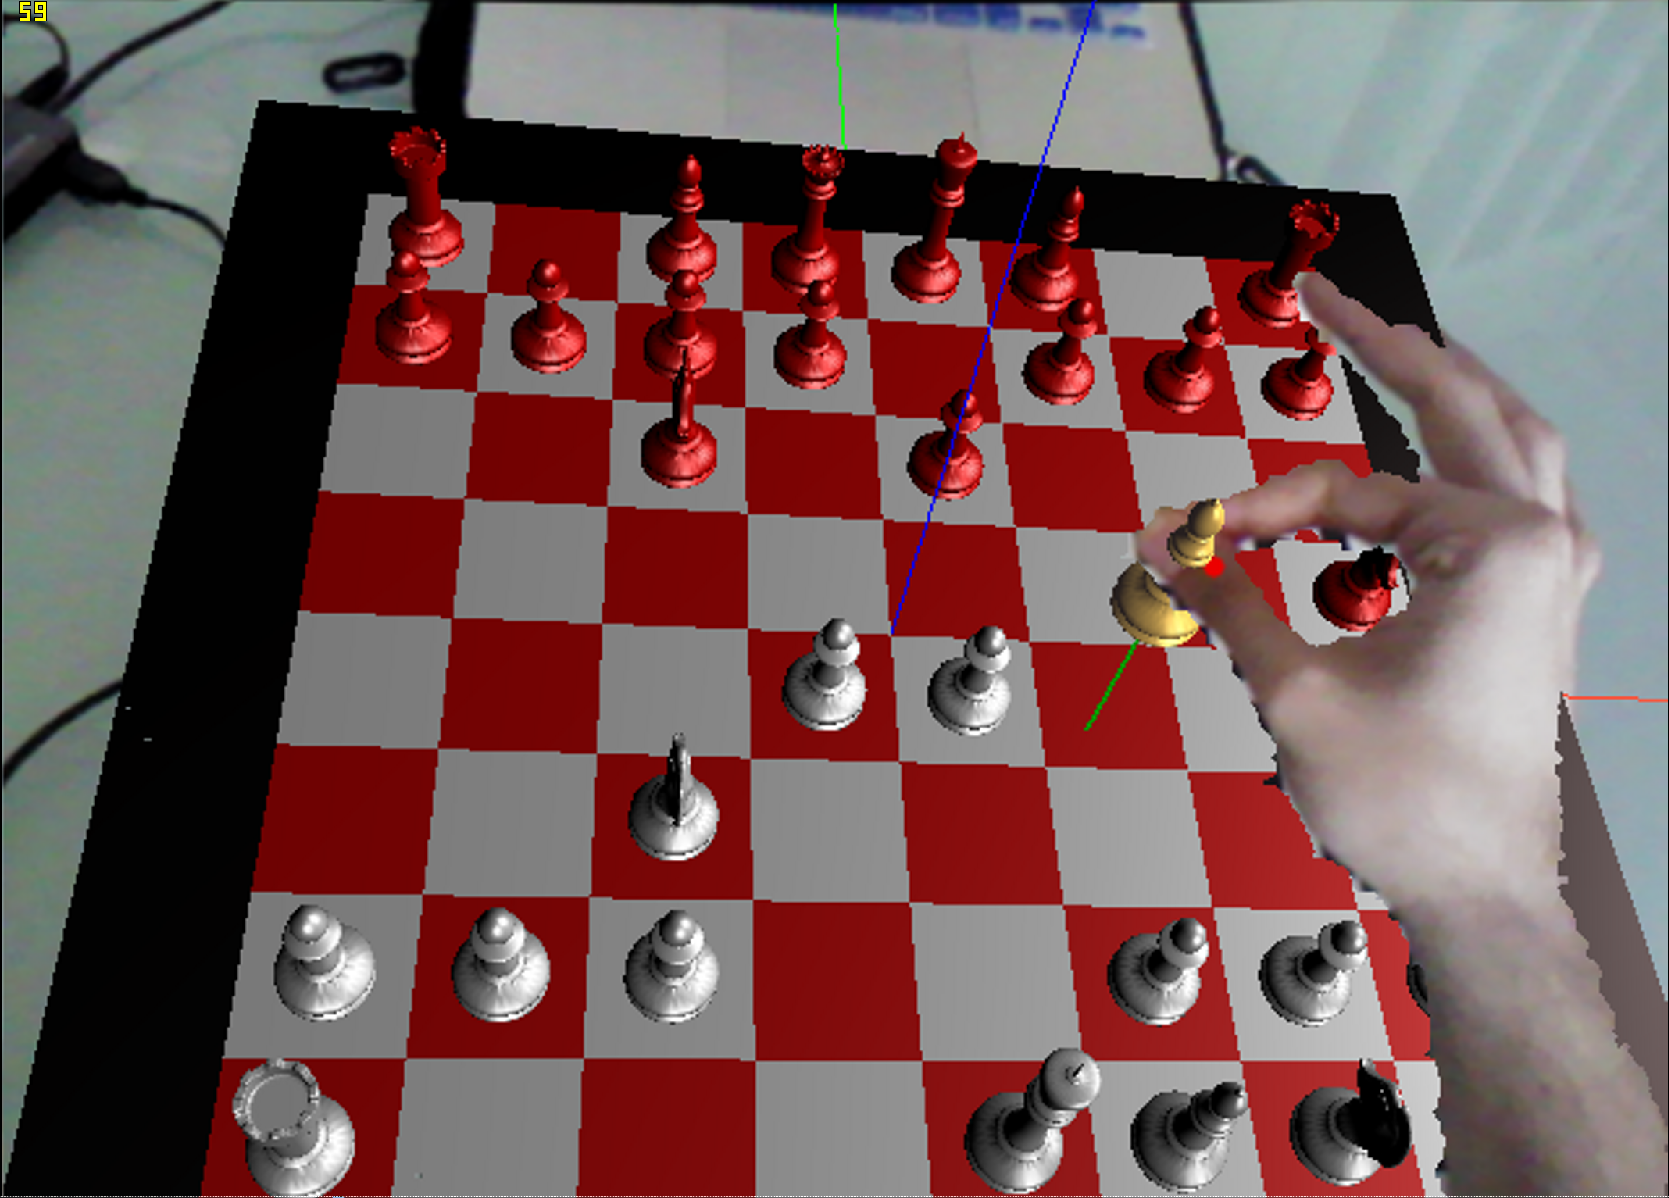
\includegraphics[width=0.55\textwidth]{Files/Figures/correct.pdf}
    \caption[Στιγμιότυπο της εφαρμογής που αναπτύχθηκε]{Στιγμιότυπο της εφαρμογής που αναπτύχθηκε}
    \label{fig:occlusion}
\end{figure}











